

\section{Evaluation}
\label{sec:eval}

%There are two goals of this sections 1) evaluate the performance of RA primitive operations Union and Join  2) evaluate the performance of transitive closure, which is a fixed point iteration algorithm.
The goal of this section is to evaluate the performance of our distributed hash-tree implementations of join, union and transitive closure at scale.
We start by individually studying the computation and communication components of the RA operations.
Computation is dominated by insertion of tuples and the major challenge faced is that of deduplication.
We therefore study the efficacy of our B-tree-based relation container in isolation.
As all our RA operations involve an all-to-all communication phase, we perform a detailed benchmark of MPI's all-to-all communication capability in isolation as well.
Finally, we benchmark the scaling properties of our distributed parallel union, join, and transitive closure operations over a range of large graphs.
%We first study how our data structure performs, and how well are the all to all communication primitives are supported by super computers. More specifically, we study how fast can we insert into our btree based relation class, and how efficiently can it support the task of de-duplication. This is mostly studying the computation aspect of our algorithms. Next, with the all to all tests, we benchmark the communication aspect of our algorithms.


%Radix-hash join and merge-sort join are two of the most popularly used parallel implementations of the inner join operation. Both these algorithms involve partitioning the input data so that they can be efficiently distributed to the participating processes. For example, in the radix-hash approach a tuple is assigned to a process based on the hash output of the column-value on which the join operation is keyed. With this approach, tuples on both relations that share the same hash value are always assigned to the same process. For every tuple in the left-hand side of the join relation is matched against all the tuples of the right-hand side of the join relation. Fast lookup data-structures like hash tables, or radix-trees (TRIE) can be used to organize the tuples within every process. The initial distribution of data using hashing reduces the overall computation overhead by a factor of the number of processes (n).

%More recently (Barthels et al. 2015, 2017), there has been a concerted effort to implement JOIN operations on clusters using an MPI backend. The commonly used radix-hash join and merge-sort join have been re-designed for this purpose. Both these algorithms involve a hash-based partitioning of data so that they are be efficiently distributed to the participating processes and are designed such that inter-process communication is minimized. In both of these implementations one-sided communication is used for transferring data between process. With one-sided communication the initiator of a data transfer request can directly access parts of the remote memory and has full control where the data will be placed. Read and write operations are executed without any involvement of the target machine. This approach of data transfer involves minimal synchronization between particiapting processes and have been shown to scale better that traditional two-sided communication. The implementation of parallel join has shown promising performance numbers; for example, the parallel join algorithm of (Barthels et al. 2017) ran successfully at 4,096 processor cores with up to 4.8 terabytes of input data

\begin{figure*}[t]
	{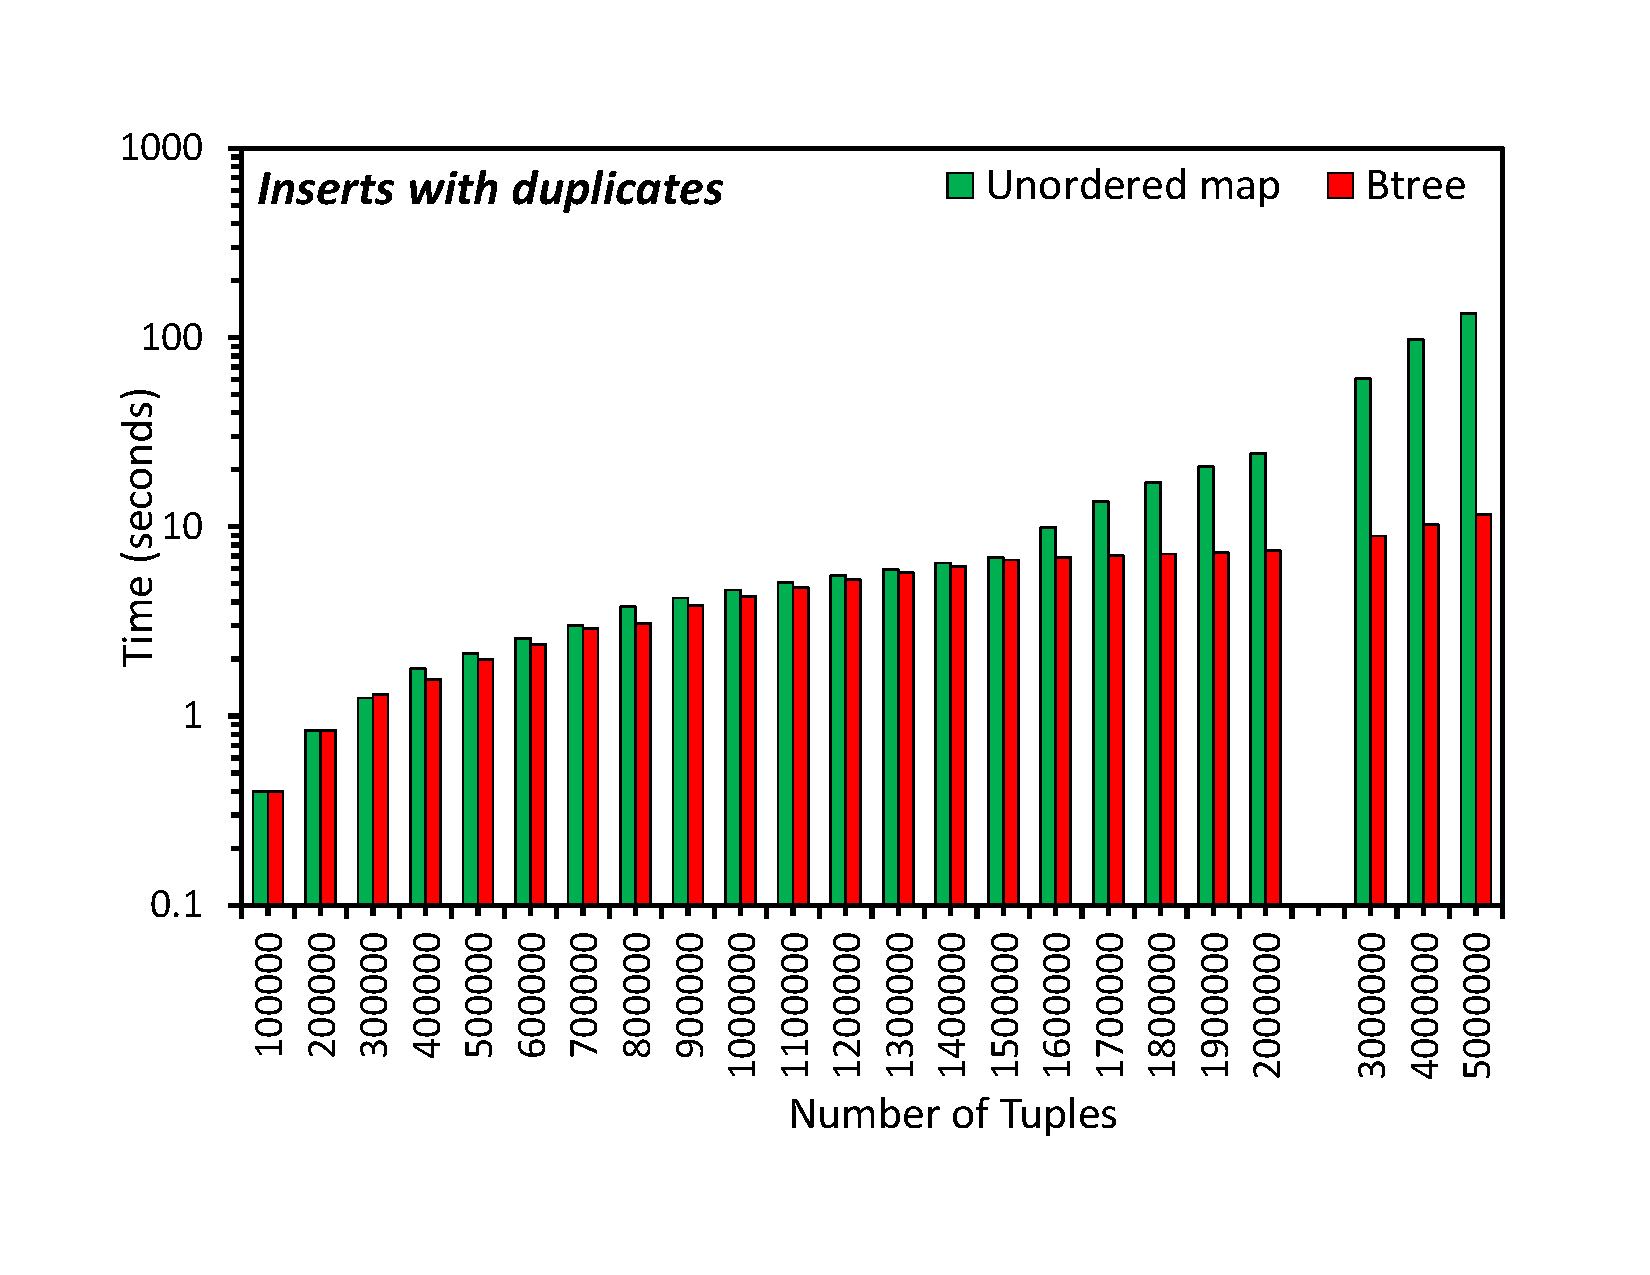
\includegraphics[width=.50\textwidth,  trim={0cm 0cm 0cm 0cm, 
			clip}]{results/inserts_with_duplicates.pdf}}\hfill%
	{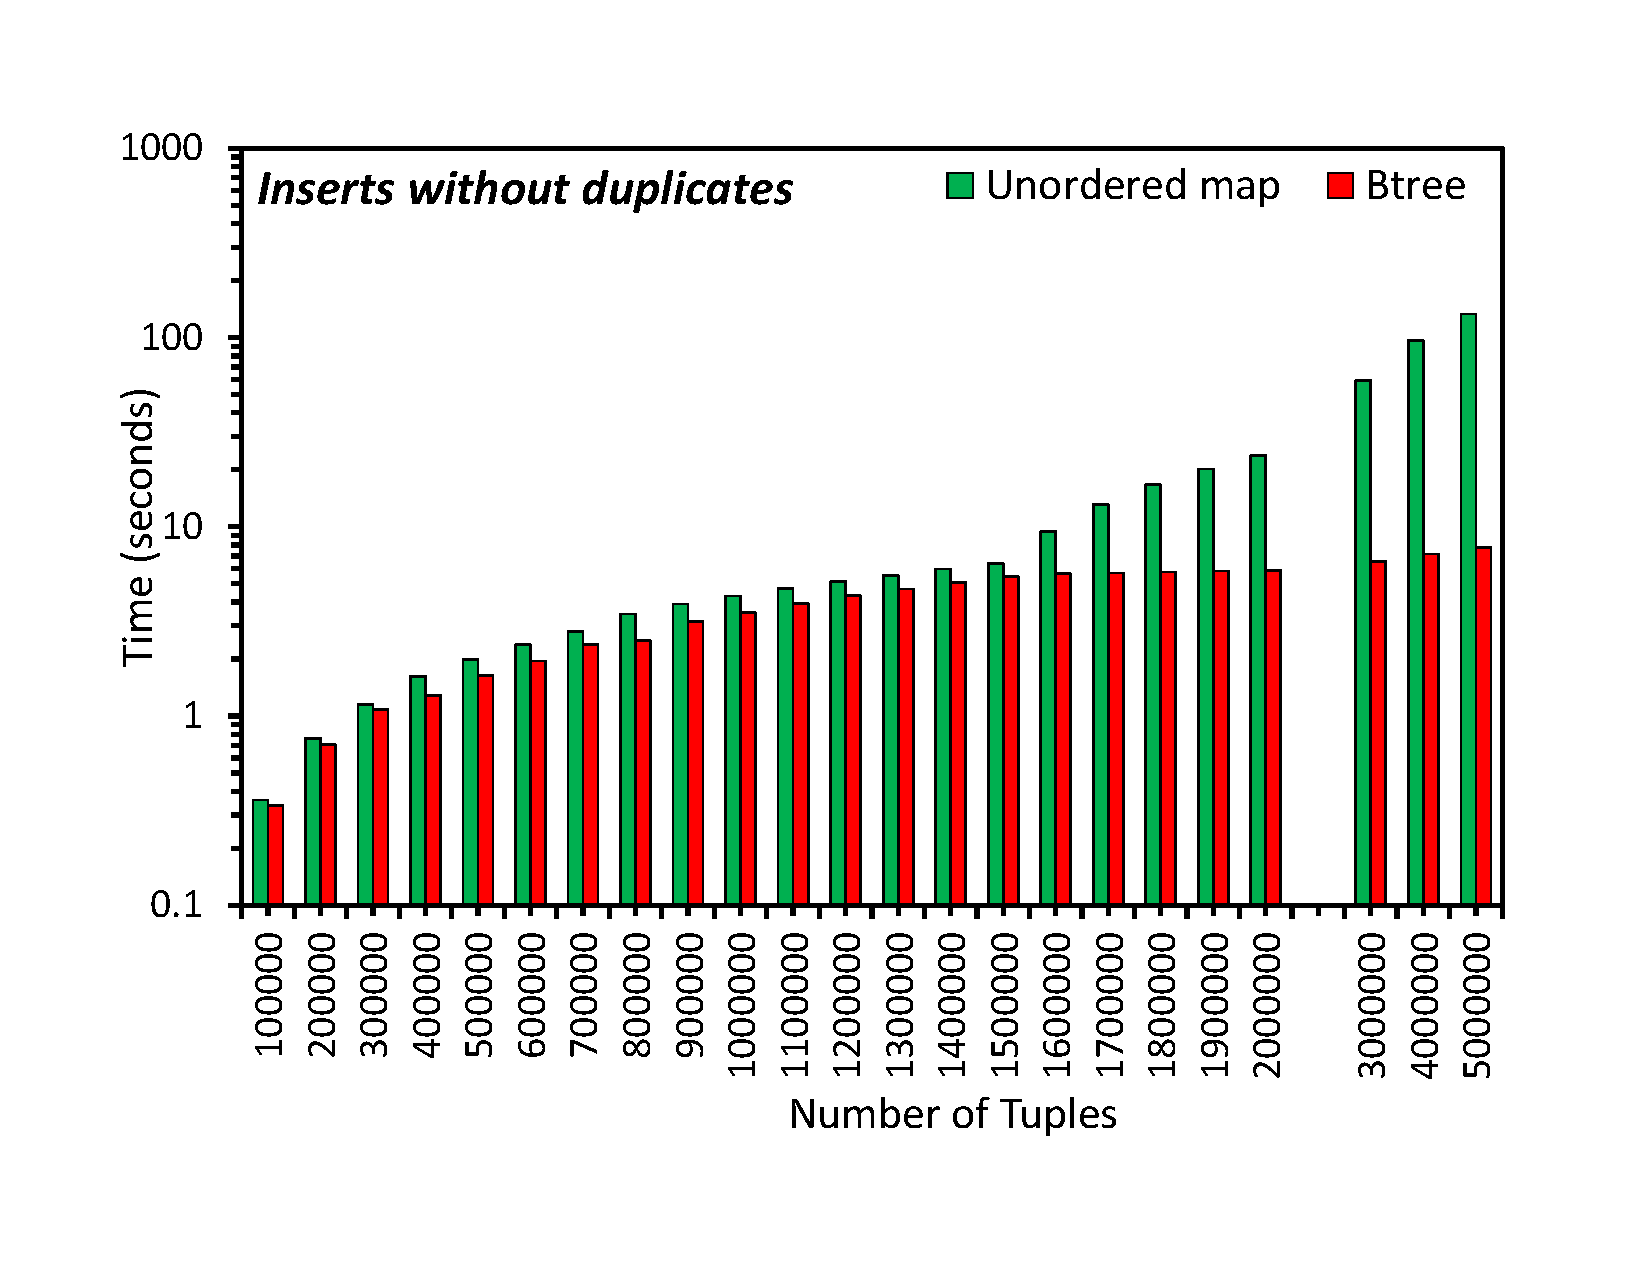
\includegraphics[width=.50\textwidth,  trim={0cm 0cm 0cm 0cm,
			clip}]{results/inserts_with_no_duplicates.pdf}}\hfill%
	\centering
	\caption{Performance evaluation of our relation class implemented as a B-tree vs unordered map. (left) All tuples are distinct; (right) There are four duplicates of every tuple. Relation implemented as a B-tree out-performs the unordered-map implementation for both cases.}
	\label{fig:tuple_inserts}
\end{figure*}


\subsection{Dataset and HPC platforms}
\label{sec:datasets}
We performed our experiments using the SuiteSparse Matrix Collection available at ~\cite{Davis:2011:UFS:2049662.2049663}.
The SuiteSparse Matrix Collection (formerly known as the University of Florida Sparse Matrix Collection), is a large and actively maintained set of sparse matrices that arise in real applications. The Collection is widely used by the numerical linear algebra community for the development and performance evaluation of sparse matrix algorithms. 
For our experiments, we chose seven graphs (listed in Table 1) representing a wide range in terms of the number of edges.
The transitive closure of a graph with $n$ edges can contain up to $n^2$ edges (a fully connected graph). The number of edges in the transitive closure of a graph depends on the connectedness and topology of the input graph. For example, the transitive closure of our third graph with $2,\!100,\!225$ edges contains $276,\!491,\!930,\!625$ edges, amounting to $4.4$ terabytes of data.

%We found our third graph with $2,100,225$ edges to be the most connected; the transitive closure of the graph generated 260 billion edges, which is 3 terabytes in size.
%-- wide range in terms of number of edges
%-- The transitive closure of third graph generated 260 billion edges, which corresponds to 4 tera bytes of data.

\begin{table}[]
	\begin{tabular}{lllll}
		\begin{tabular}[c]{@{}l@{}}Input graph \\ edge count\end{tabular} & Union & Join & \begin{tabular}[c]{@{}l@{}}Transitive \\ Closure\end{tabular} \\
		\hline
		412148     & \checkmark       &      &  1676697757 \\
		2100225    & \checkmark       &      &  276491930625\\
		6291408    & \checkmark       &      &  308759592                \\
		40451631   & \checkmark       &      &  --   			              \\
		59062957   & \checkmark       &      &  11687744437        \\
		136024430  & \checkmark       & \checkmark     & 178113958 \\
		180292586  & \checkmark       & \checkmark      &136525288391 \\
%		240023949  & 			      &      &  --                                                             &           
	\end{tabular}
	\label{table:graph1}
	\caption{List of seven graphs used in our evaluation. Also listed is the number of edges in the transitive closure of every graph.}
\end{table}



%a Cray machine with Intel Xeon Phi processors with Dragonfly topology network and Lustre file system [31].

The experiments presented in this work were performed on
the Theta Supercomputer at the Argonne Leadership Computing Facility
(ALCF). Theta is a Cray machine with a peak
performance of $11.69$ petaflops, $281,\!088$ compute cores, $843.264$
TiB of DDR4 RAM, $70.272$ TiB of MCDRAM and $10$ PiB of online disk storage. 
The supercomputer has Dragonfly network topology and a Lustre filesystem.

%Default striping was used with the Lustre file system. Mira system contains 48 racks and 768K cores, and has a theoretical peak performance of 10 petaflops. Each node has 16 cores, with 16 GB of RAM per node. I/O and interprocessor communication travels on a 5D torus network. Every 128 compute nodes has two 2 GB/s bandwidth links to two different I/O nodes, making 4 GB/s bandwidth for I/O at most. I/O nodes are connected to file servers through QDR IB. Mira uses a GPFS file system with 24 PB of capacity and 240 GB/s bandwidth.


\subsection{Relation container}
\label{sec:relation}

In this section we evaluate the efficacy and scaling of our per-bucket relation container. We measure performance for two cases: insertions of unique tuples and insertions of tuples with duplicates. In the later set of experiments, each tuple had four duplicates. For both sets of experiments, we compare two implementations of the relation class, one with our B-tree back-end and the other with a hash table back-end. For the hash table experiments, we used \texttt{unordered\_map} from C++'s standard template library. The results can be seen in Figure~\ref{fig:tuple_inserts}. The x-axis corresponds to the total number of tuples being inserted (successfully) and the y-axis is the time taken for this task to finish. We observe that our B-tree-based relation container outperforms the hash-table-based implementation for insertion of all tuple counts. Furthermore, the hash-table-based relation container fails to scale with the insertion of a very large number of tuples. For example, the hash-based relation takes $59.45$ seconds to insert $3000000$ tuples as opposed to only $6.58$ seconds taken by the B-tree-based relation. Similar results can be observed for insertion of tuples with duplicates. The B-tree-based relation container successfully deduplicates tuples while maintaining high performance.
%To facilitate fast inserts and lookups of tuples, we implemented a relation container.
%We made two implementations of the container one using btrees and other using unordered\_map from the standard template library.
%The relation container is a recursive, nested data-structure. \textbf{More stuff.}
%, for example, for two-tuple we have a btree with keys as the first column-entries, and the value is a new btree which is again
%Deduplication is a major challenge while inserting tuples, for example, join between two relation followed by projection of the common column often yields a lot of duplicate tuples. 


%-- Perform two benchmarks: insertion of tuples without any duplicate and insertion of tupes each with four duplicates.
%-- Relation class implemented with btrees outperforms relation with hashes.
%-- 



\begin{figure*}[t]
	{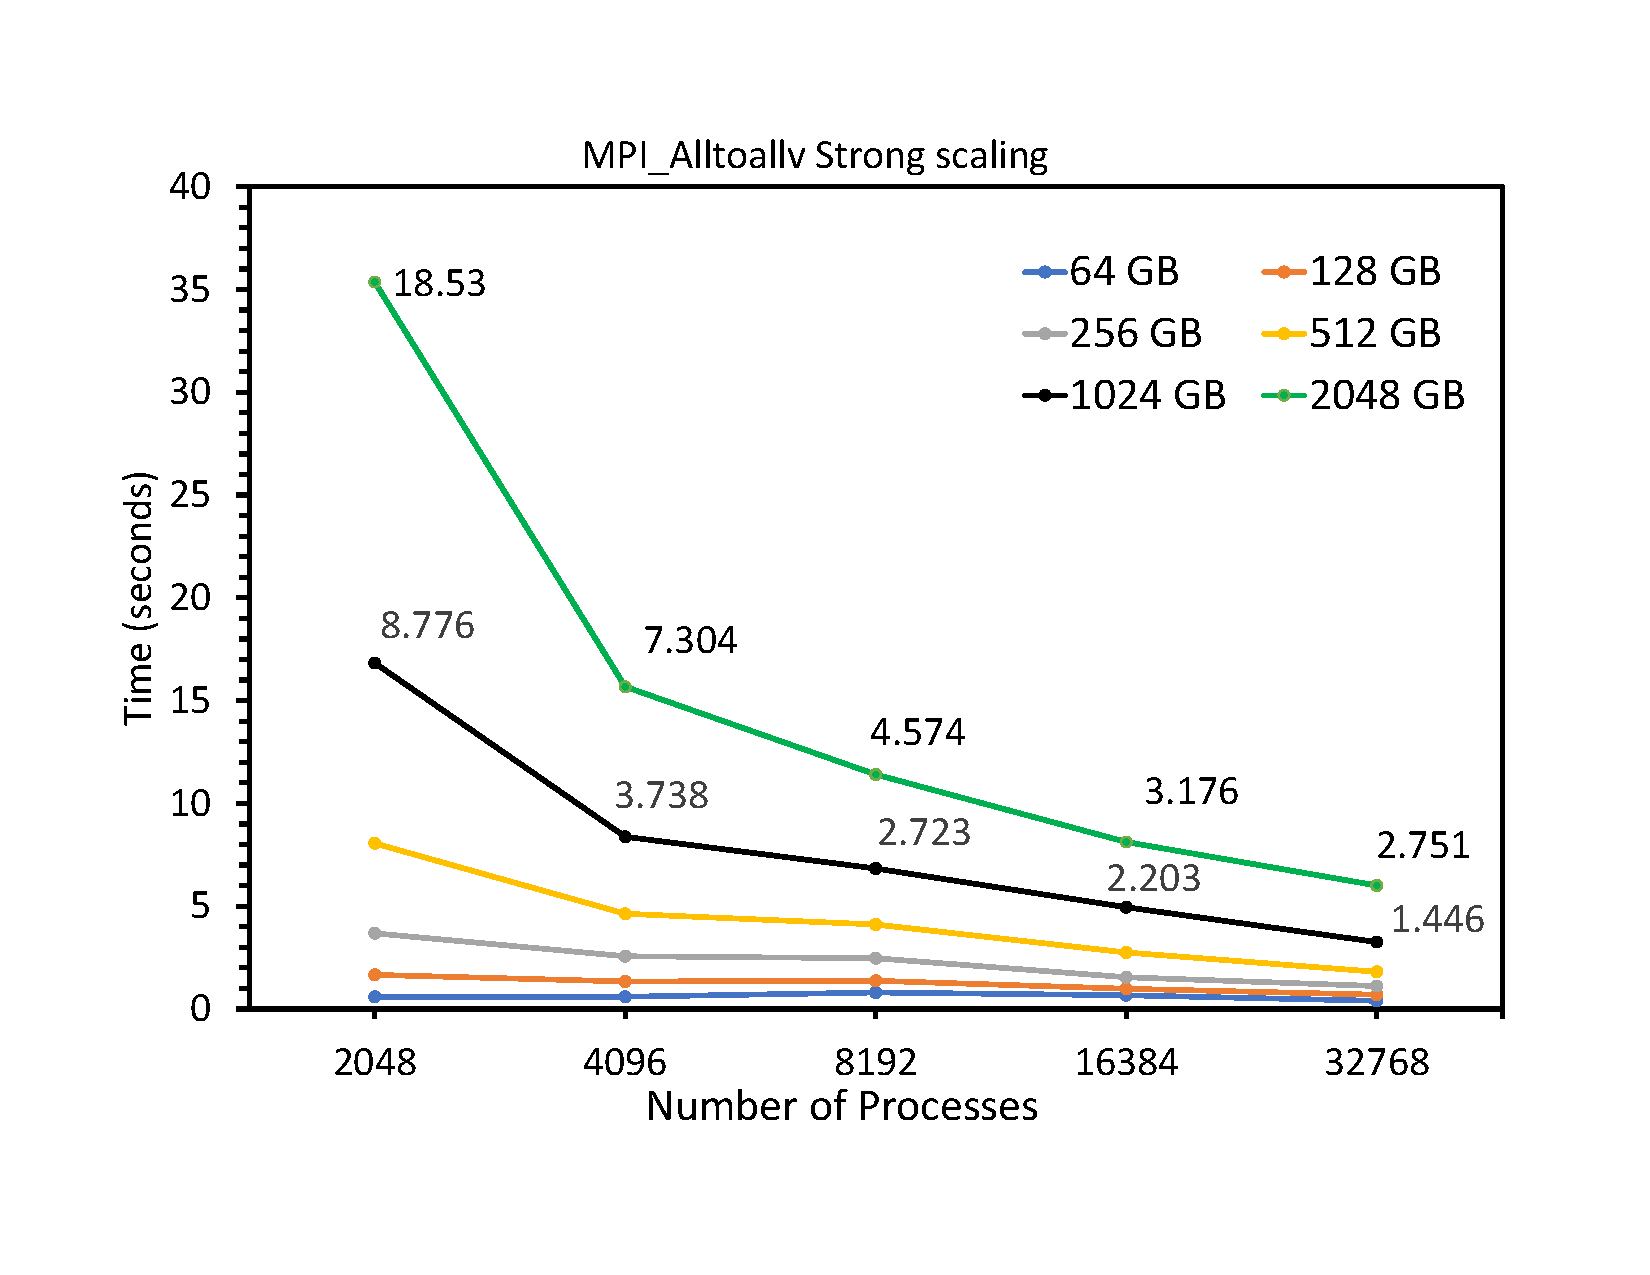
\includegraphics[width=.50\textwidth,  trim={0cm 0cm 0cm 0cm, 
			clip}]{results/all_to_all_strong.pdf}}\hfill%
	{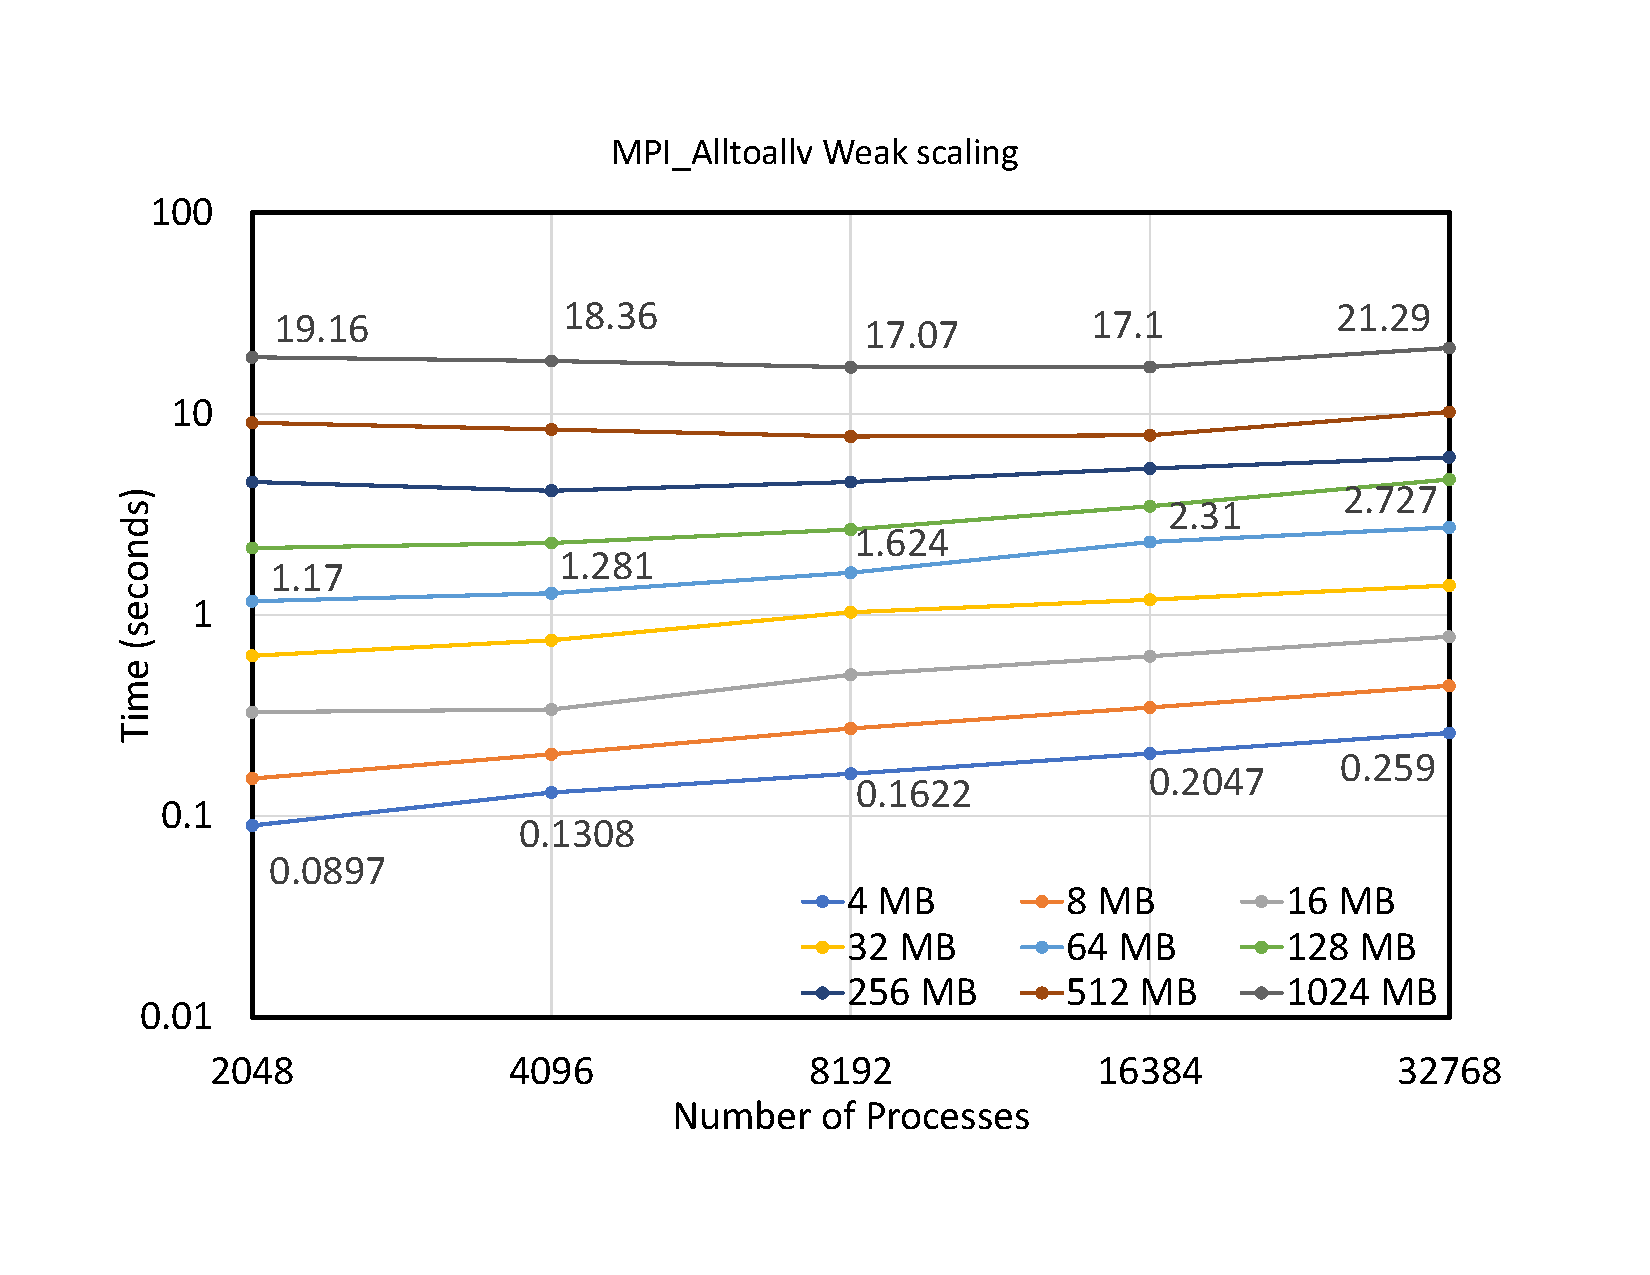
\includegraphics[width=.50\textwidth,  trim={0cm 0cm 0cm 0cm,
			clip}]{results/all_to_all_weak.pdf}}\hfill%
	\centering
	\caption{Strong (left) and Weak (right) scaling evaluation of MPI\_alltoallv function of MPI. }
	\label{fig:all_to_all}
\end{figure*}


\subsection{MPI\_All\_to\_Allv}
\label{sec:all_to_all}


%All our RA operations require all to all communication.
All-to-all communication is central to all of our distributed RA algorithms (Section~\ref{sec:impl}).
We use MPI's MPI\_Alltoallv function to facilitate all-to-all data communication.
MPI\_Alltoallv transmits data between all pairs of processes where each process can send a variable amount of data by providing offsets for the input and output data. In this section we study both weak and strong scaling characteristics of MPI\_Alltoallv.
For both sets of experiments, we varied the number of processes from $2,\!048$ to $32,\!768$. We performed $9$ sets of weak scaling experiments. For these $9$ experiments, the amount of data transmitted by each process ($data_{process}$) was varied from $4$ megabytes (in the $1\textsuperscript{st}$ set) to $1,024$ megabytes (in the $9\textsuperscript{th}$ set). For an $n$-process run, every process transmits $\mathit{data}_\mathit{process}/n$ units of data to every other process. For strong scaling experiments, we performed 6 sets of experiments, varying the total amount of data generated across processes ($data_{total}$) from $64$ gigabytes (in the $1\textsuperscript{st}$ set) to $2,\!048$ gigabytes (in the $6\textsuperscript{th}$ set). The amount of data generated by every process is the same; for example, for an $n$-process run, and $\mathit{data}_\mathit{total}$ units of data, every process produces $\mathit{data}_\mathit{total}/n$ units of data. A process then transmits $\mathit{data}_\mathit{total}/{n^2}$ units of data to every other process. The results of both weak and strong scaling experiments can be seen in Figure~\ref{fig:all_to_all}.

For both strong and weak scaling runs, we observe a decline in performance with overall decreasing workload. For instance, with strong scaling, the $6$\textsuperscript{th} set of experiments, where total workload is $2,048$ gigabytes, shows near perfect scaling when the number of processes is doubled from $2,\!048$ ($18.5$ seconds) to $4,\!096$ ($7.3$ seconds) to $8,\!192$ ($4.5$ seconds). After $8,192$ processes, although total time continues to come down with increasing process count, we observe that the rate of improvement drops off. Furthermore, looking at the $6$\textsuperscript{th} set of experiments, where total workload is $64$ gigabytes, we observe relatively poor scaling characteristics across the entire process range. Both these observations may be attributed to an overall reduction in per-process workload. With less data to transmit, total time is dominated by initialization costs as opposed to actual data-transmission cost. For example, with total workload of $64$ gigabytes, at $4,096$ processes, every process gets a workload of only $16$ megabytes ($64$ gigabytes $/ 4096$), and ends up sending $8$ kilobytes ($16$ megabytes $/ 4096$) of data to every other process. Similarly, for weak scaling experiments as well, when the amount of data exchanged is substantial, we see almost perfect scaling. For example, when the amount of data transmitted by every process is $1024$ megabytes, we observe almost perfect scaling, whereas when the amount of data sent by every process is small (e.g., $4$ megabytes) we observe poor scaling.

In the context of communication requirements for distributed RA operations, we find the scaling trends of MPI\_alltoallv to be encouraging. In general, for a given workload (i.e., overall tuple count for RA operations), there will always be a range of processes that exhibits good all-to-all scaling characteristics. What remains is the challenge of identifying the ideal process count to balance the trade-off between computation and communication. As we observe in section~\ref{sec:tc}, below, with larger per-process workload computation cost dominates, as opposed to smaller per-process workload where total cost is dominated by communication. 
%As we will ee later the crucial part will be to identify the process count that balances computation and communication in the monst efficient way.

%For every input graph, we need to find the range of process count that exhibits 
%The trends suggests that there is a range of process count suitable for different graphs. There is a window of process count suitable for graphs of differeing sizes. As the number of processes increases the amount of data (tuples) held by every process starts t

%-- perform both weak and strong scaling
%-- configuration
%-- weak scaling with accuracy X percent accuracy for per process load of Y versus Z percent accuracy for per process load of M.
%-- Exhibit poor weak scaling for small load, as opposed to good weak scaling with larger volume of data.
%-- X percent accuracy with strong scaling of X load. This corresponds to Y number of tuples.
%-- Overall very good indication as all to all scales well, aggregate accuracy
%-- different graphs would work better at different scales.

\subsection{Distributed Union}
\label{sec:union}

%\begin{figure*}[t]
%	{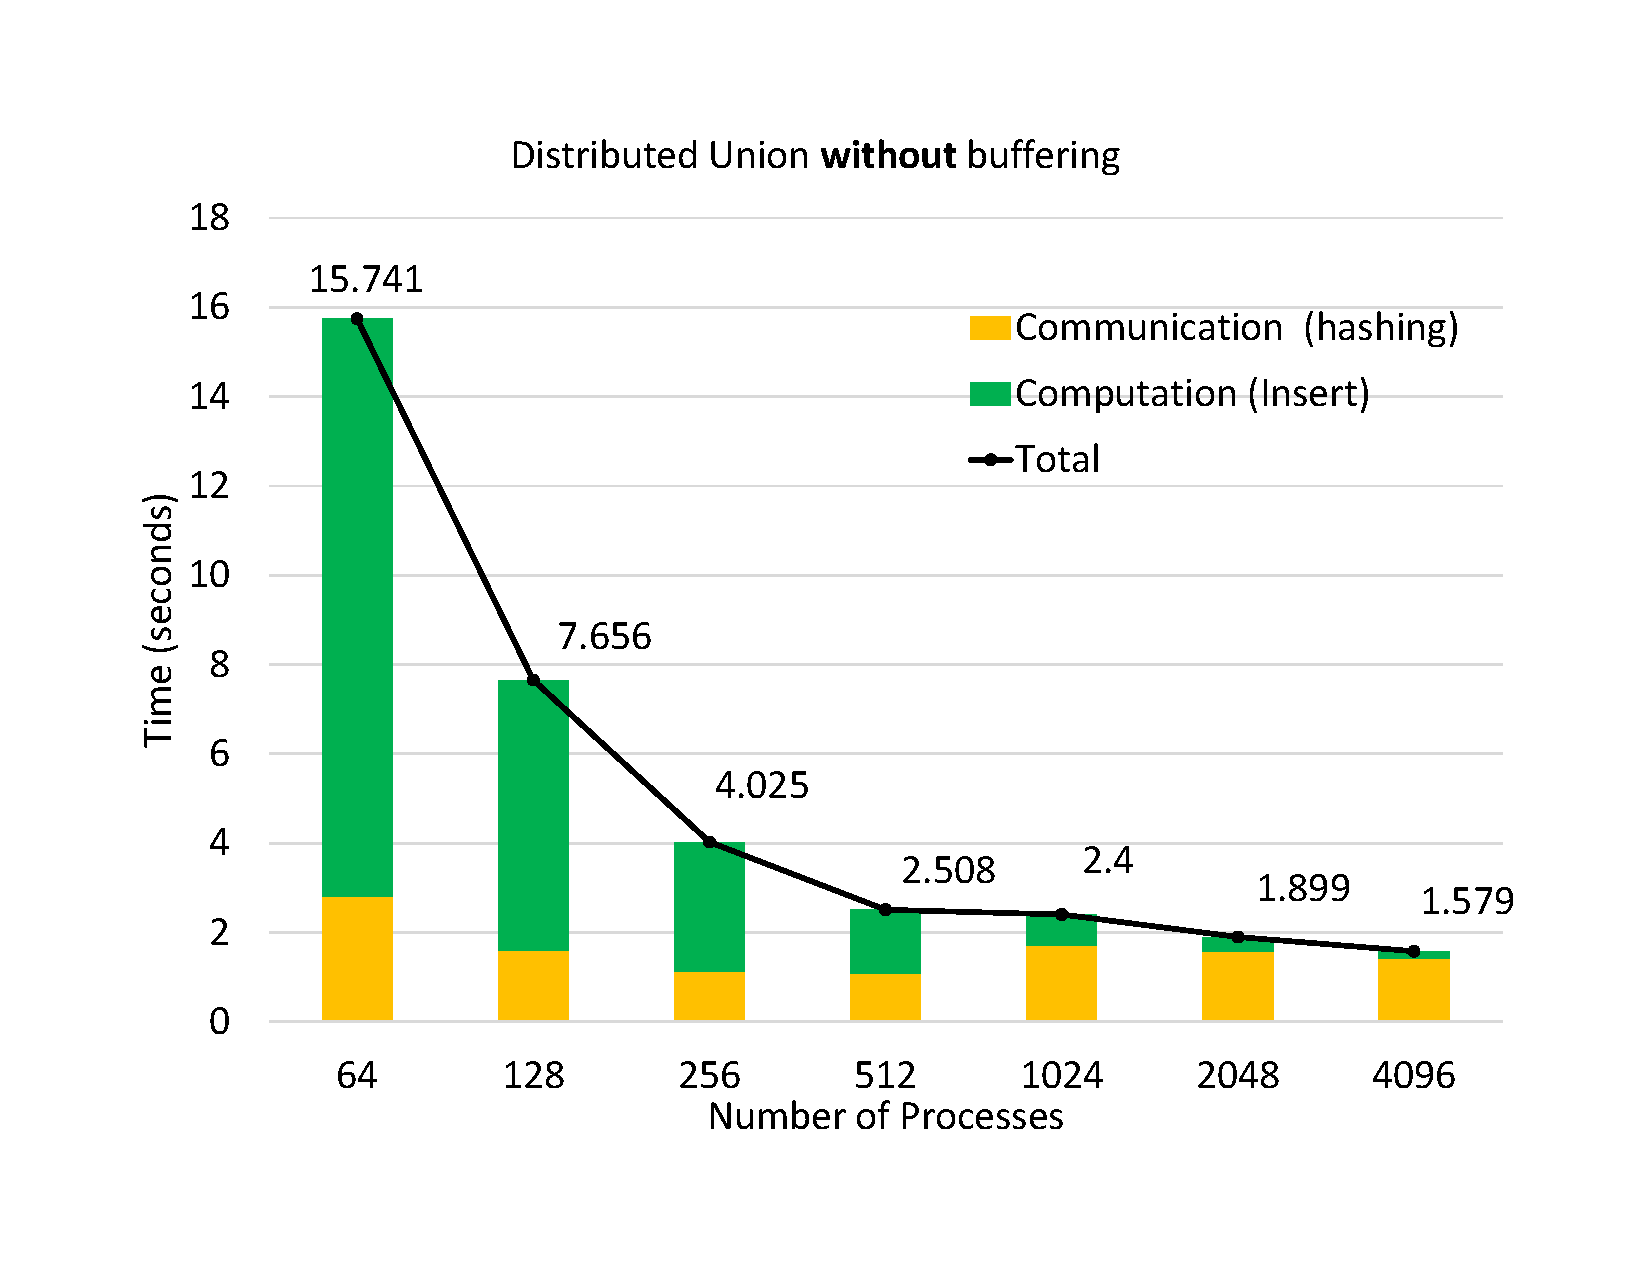
\includegraphics[width=.50\textwidth,  trim={0cm 0cm 0cm 0cm, 
%			clip}]{results/union_without_buffering_final.pdf}}\hfill%
%	{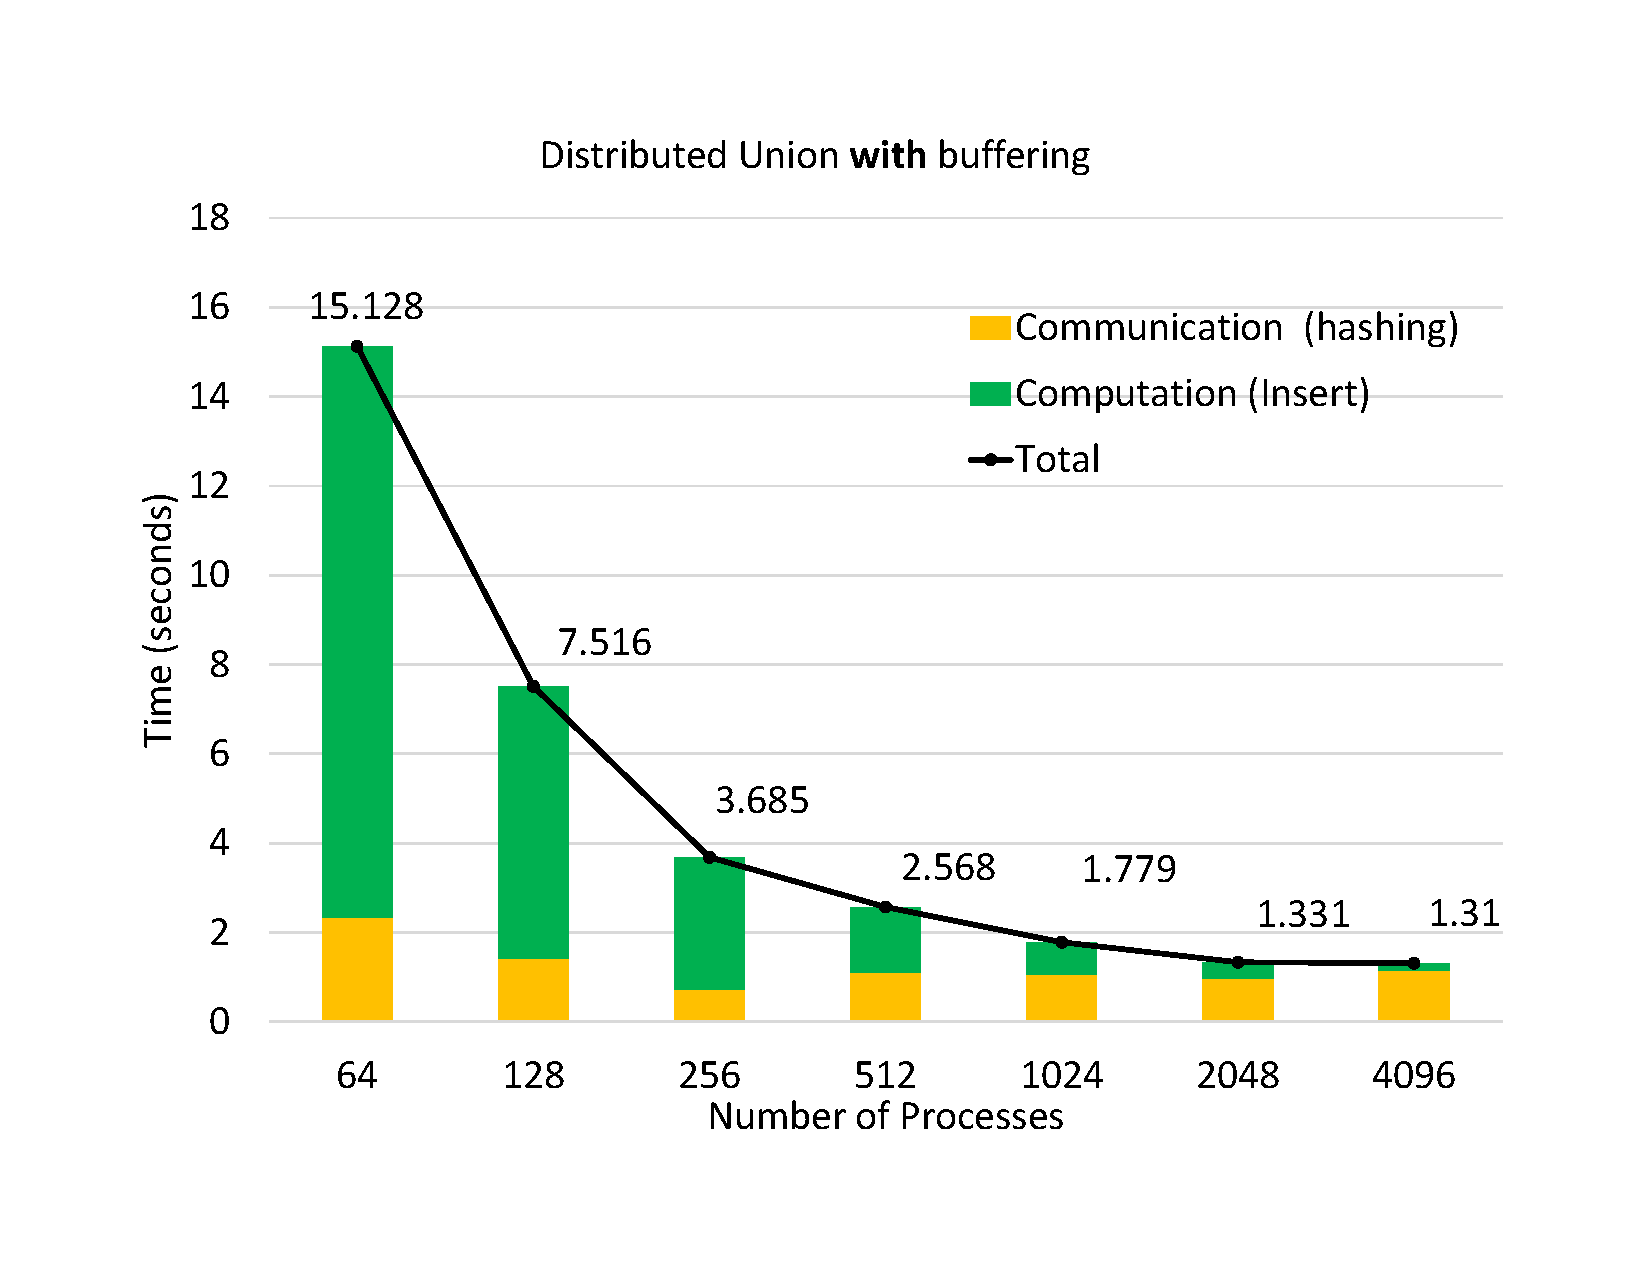
\includegraphics[width=.50\textwidth,  trim={0cm 0cm 0cm 0cm,
%			clip}]{results/union_with_buffering_final.pdf}}\hfill%
%	\centering
%	\caption{Distributed union.}
%	\label{fig:dist_union}
%\end{figure*}

We examine strong scaling to benchmark the performance of our distributed hash-tree union. We measure the time to union $7$ graphs listed in table 1. The number of processes are varied from $64$ to $4,\!096$. The total number of edges across all $7$ graphs is $664,\!659,\!334$ ($9.9$ gigabytes of data). The union of all $7$ graphs has $424,\!592,\!810$ edges, indicating significant overlap among the graphs.

\begin{figure}[h]
	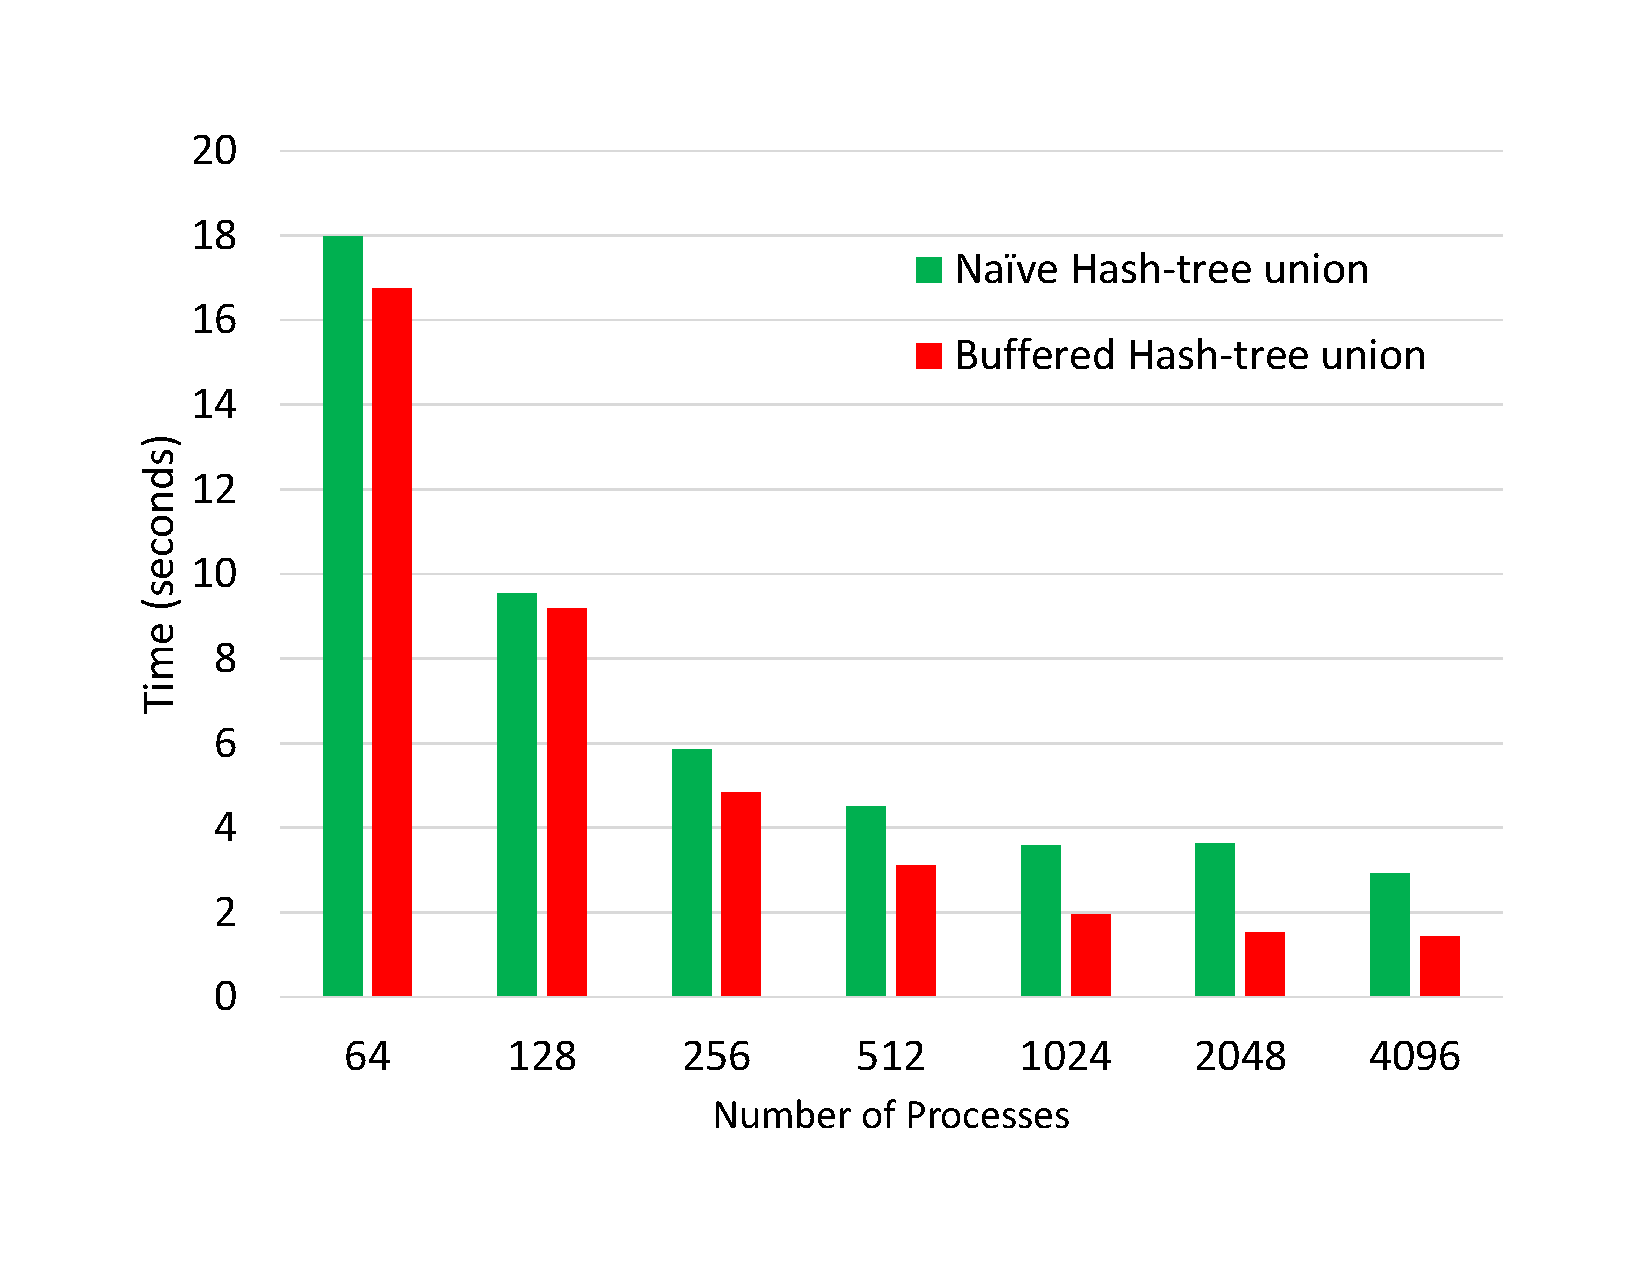
\includegraphics[width=\columnwidth]{results/hash_tree_union.pdf}
	\caption{Strong scaling result of hash-tree union.}
	\label{fig:dist_union}
\end{figure}

We benchmark the performance of both buffered hash-tree join and na\"ive hash-tree join. 
Performance of both techniques can be seen in Figure~\ref{fig:dist_union}. We observe two trends: at all process counts, buffered hash-tree union outperforms na\"ive hash-tree union. This trend can be attributed to an optimized data communication phase associated with buffered unions. Na\"ive one-by-one union leads to communication involving a small number of large-sized data packets as opposed to the buffered union that involves communication with a large number of small-sized data packets. 
The other crucial trend is that the union phase only scales to $1024$ cores, this can be attributed to an increase in communication time at higher core counts associated with movement of many small-sized data packets. This result corroborates the trend seen in Section~\ref{sec:all_to_all}. At $2,\!048$ and $4,\!096$ processes, even though the insertion time is reduced, the per-process workload becomes small, impeding scalability of the communication phase. 

It can be concluded that for this particular union task ($7$ graphs) $1024$ is the ideal degree of parallelism, as that balances the communication and computation tasks best.

%This step is followed by 

%-- union of 7 graphs from table
%-- union comprises of an io phase followed by communication and then followed by inserts
%-- We compare two union types, one is where we perform io, comm and compute separates, the other is where we first perform io for all and then we bundle all our comm and then we have one phase of compute
%-- scales well upto X cores., this is strong scaling.
%-- faces work load deprecation at low core counts, needs more tuples for union to scale at high core counts
%-- overall a good sign


\subsection{Distributed Join}
\label{sec:join}

\begin{figure}[h]
	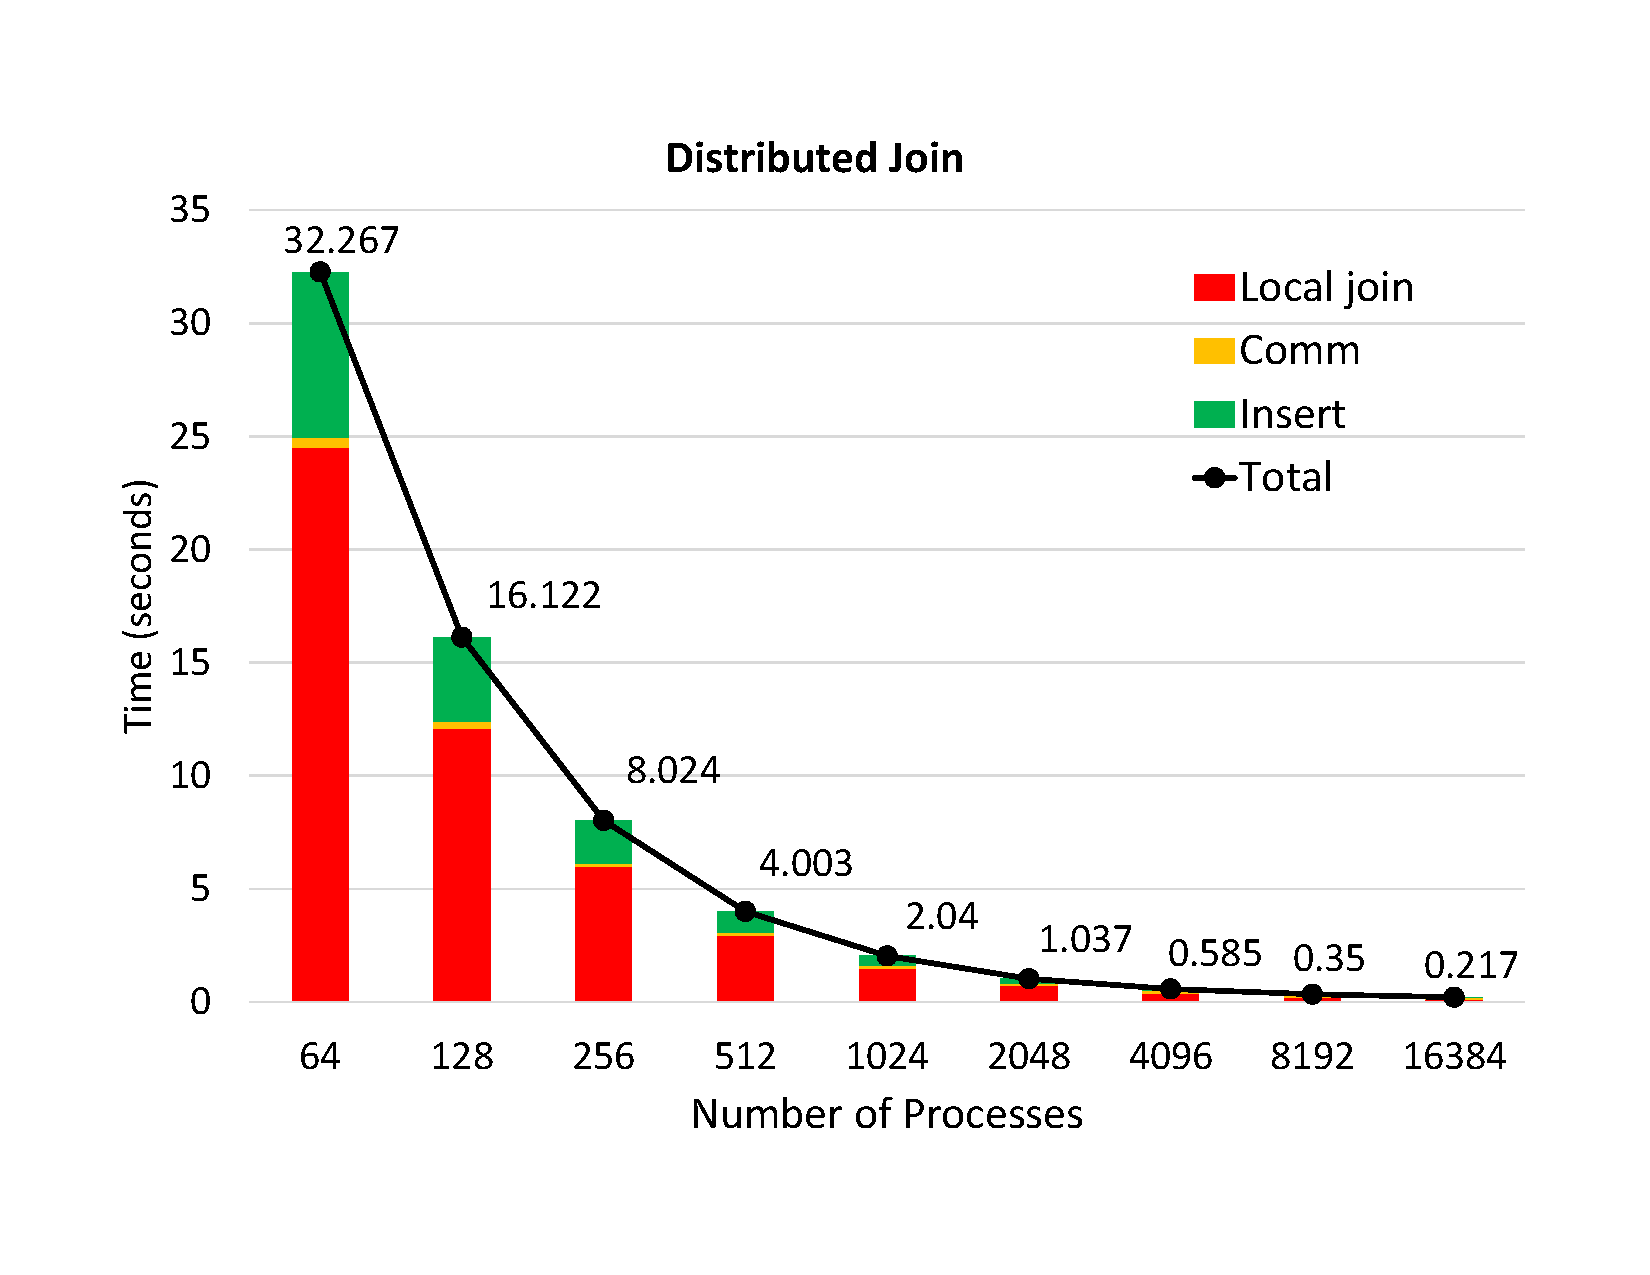
\includegraphics[width=\columnwidth]{results/join_new_final.pdf}
	\caption{Strong scaling result of hash-tree join.}
	\label{fig:dist_join}
\end{figure}

As with distributed union, we examine strong scaling to benchmark the performance of our distributed join.
We perform hash-tree join between two graphs with edge counts $136,\!024,\!430$ and $180,\!292,\!586$. The join operation yields a graph with $126,\!290,\!622$ number of edges.
The number of processes are varied from $64$ to $16,384$. 
%Unlike union, where we maintained only one relation container for all input graphs, here we have separate relation containers for the two input graphs. 
Once both relations are initialized across all processes (after parallel I/O, hashing, communication and insertions), we initiate the join operation. 
We plot the scaling results for join in Figure~\ref{fig:dist_join}.
%We observe trends similar to distributed union.
Unlike unions, distributed joins demonstrates perfect scaling all the way to $4096$ processes. At $4096$ processes join between the two graphs takes $0.575$ seconds. The trend can be attributed to the fact all-to-all communication phase continues to scale till $4096$ processes.
Though it stops to scale after $4096$ processes, leading to slight dip in performance at $8,192$ and $16,384$ processes.


%Join only scales up to X cores, after which communication cost starts to dominate and we observe overall decline in performance. %% Do we really see any decline? Up to 4k it still looks great!


\subsection{Transitive closure}
\label{sec:tc}

In this section we benchmark a transitive closure computation using our distributed RA and the algorithm discussed in section~\ref{sec:impl}.
The transitive closure ($T$) of an input graph ($G$) is iteratively extended by adding new paths discovered by a join operation until a fixed point is reached, and no new paths can be added to $T$.
Every iteration is comprised of four phases: 1) a local join 2) all-to-all network communication 3) insertion of new tuples 4) checking if a fixed point was reached.

% In the local join phase every process concurrently computes the join of relations $G$ and $T = \rho_{0 / 1}(G)$ which creates new edges. Following the semi-naive evaluation (discussed in Section~\ref{}), the new edges then need to be added back to relation $T$. This step of adding the newly created edges to T, entails all to all communication, as the new new edges need to be rehashed and transmitted to the appropriate process (hash-bucket). This all-to-all communication is accomplished using MPI’s MPI\_alltoallv. Once the new edges arrive at a process they are inserted to Following the insertion phase, the newly created edges are inserted to the relation T. In the final step we check if the size of the relation $T$ changed on any process, if it does then we have not yet reached a fixed point and we continue to another iteration of these 4 steps.

We performed detailed strong scaling analysis for two graphs, with edge count $412,\!148$ (graph $G1$) and $2,\!100,\!225$ (graph $G2$).
For $G1$ we varied the number of processes from $64$ to $8,\!192$, while for $G2$ we varied the number of processes from $4,096$ to $65,\!536$. 
$G1$ attained its fixed point after $2,\!933$ iterations, generating a total of $1,\!676,\!697,\!415$ edges ($25$ gigabytes).
$G2$ attained its fixed point after $2,\!956$ iterations, generating a total of $276,\!491,\!930,\!625$ edges $(4 terabytes)$.
The results for graph $G1$ and $G2$ are respectively plotted in Figure~\ref{fig:tc_small} and Figure~\ref{fig:tc_big}. As can be seen in the Figure~\ref{fig:tc_big}, our approach takes $922$ seconds at $65,\!536$ cores to compute the transitive closure of graph $G2$. To the best of our knowledge, this is the first implementation that has successfully computed the transitive closure of such a large graph.

Further, looking at the graph we obtain for $G1$ we observe considerable scaling up to $1,024$ processes; for $2,048$ and $4,096$ processes, the runs are completely dominated by communication time. This observation again corroborates our strong scaling benchmarking results, where all-to-all communication stops scaling in the presence of many small-sized data packets. For $G1$ we can conclude that $1024$ is the ideal scale for computing transitive closure.
We observe similar trend with graph $G2$: communication time begins to dominate performance at high core counts of $32,\!768$ and $65,\!536$. %%~\textbf{more stuff, conclude}


%seconds at 64 cores and 235 seconds at 2048 cores, corresponds
%to an overall efficiency of 6.25%. We investigated these timings further by plotting the timing breakdown
%of by the four major components (join, network communication, join, fixed-point check) of the algorithm. We
%observe (see Figure 2) that for all our runs the total time is dominated by computation rather than communication;
%insert and join together tended to take up close to 90% of the total time. This is quite an encouraging result
%as it shows that we are not bound primarily by the network bandwidth (at these scales and likely moderately
%higher ones) and it gives us the opportunity to optimize the computation phase

\begin{figure*}[t]
	{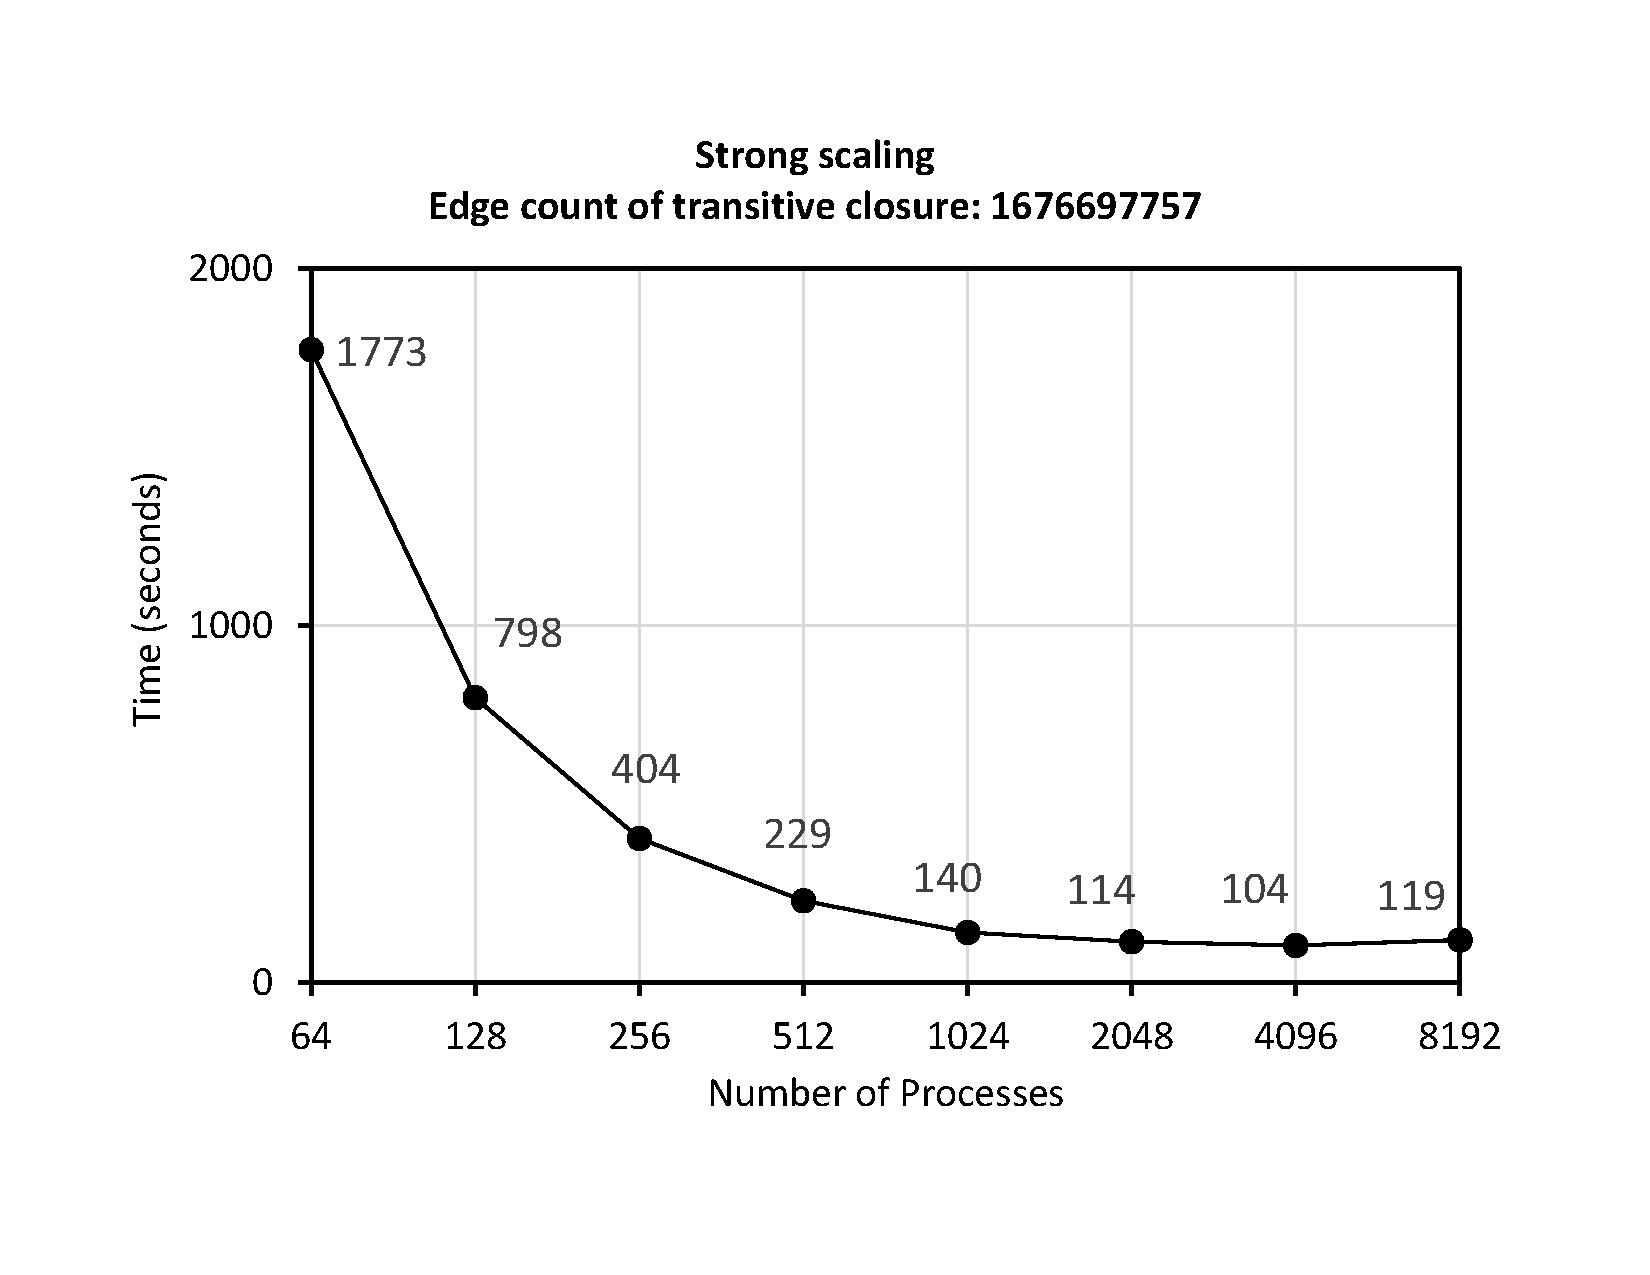
\includegraphics[width=.50\textwidth,  trim={0cm 0cm 0cm 0cm, 
			clip}]{results/TC_1_final.pdf}}\hfill%
	{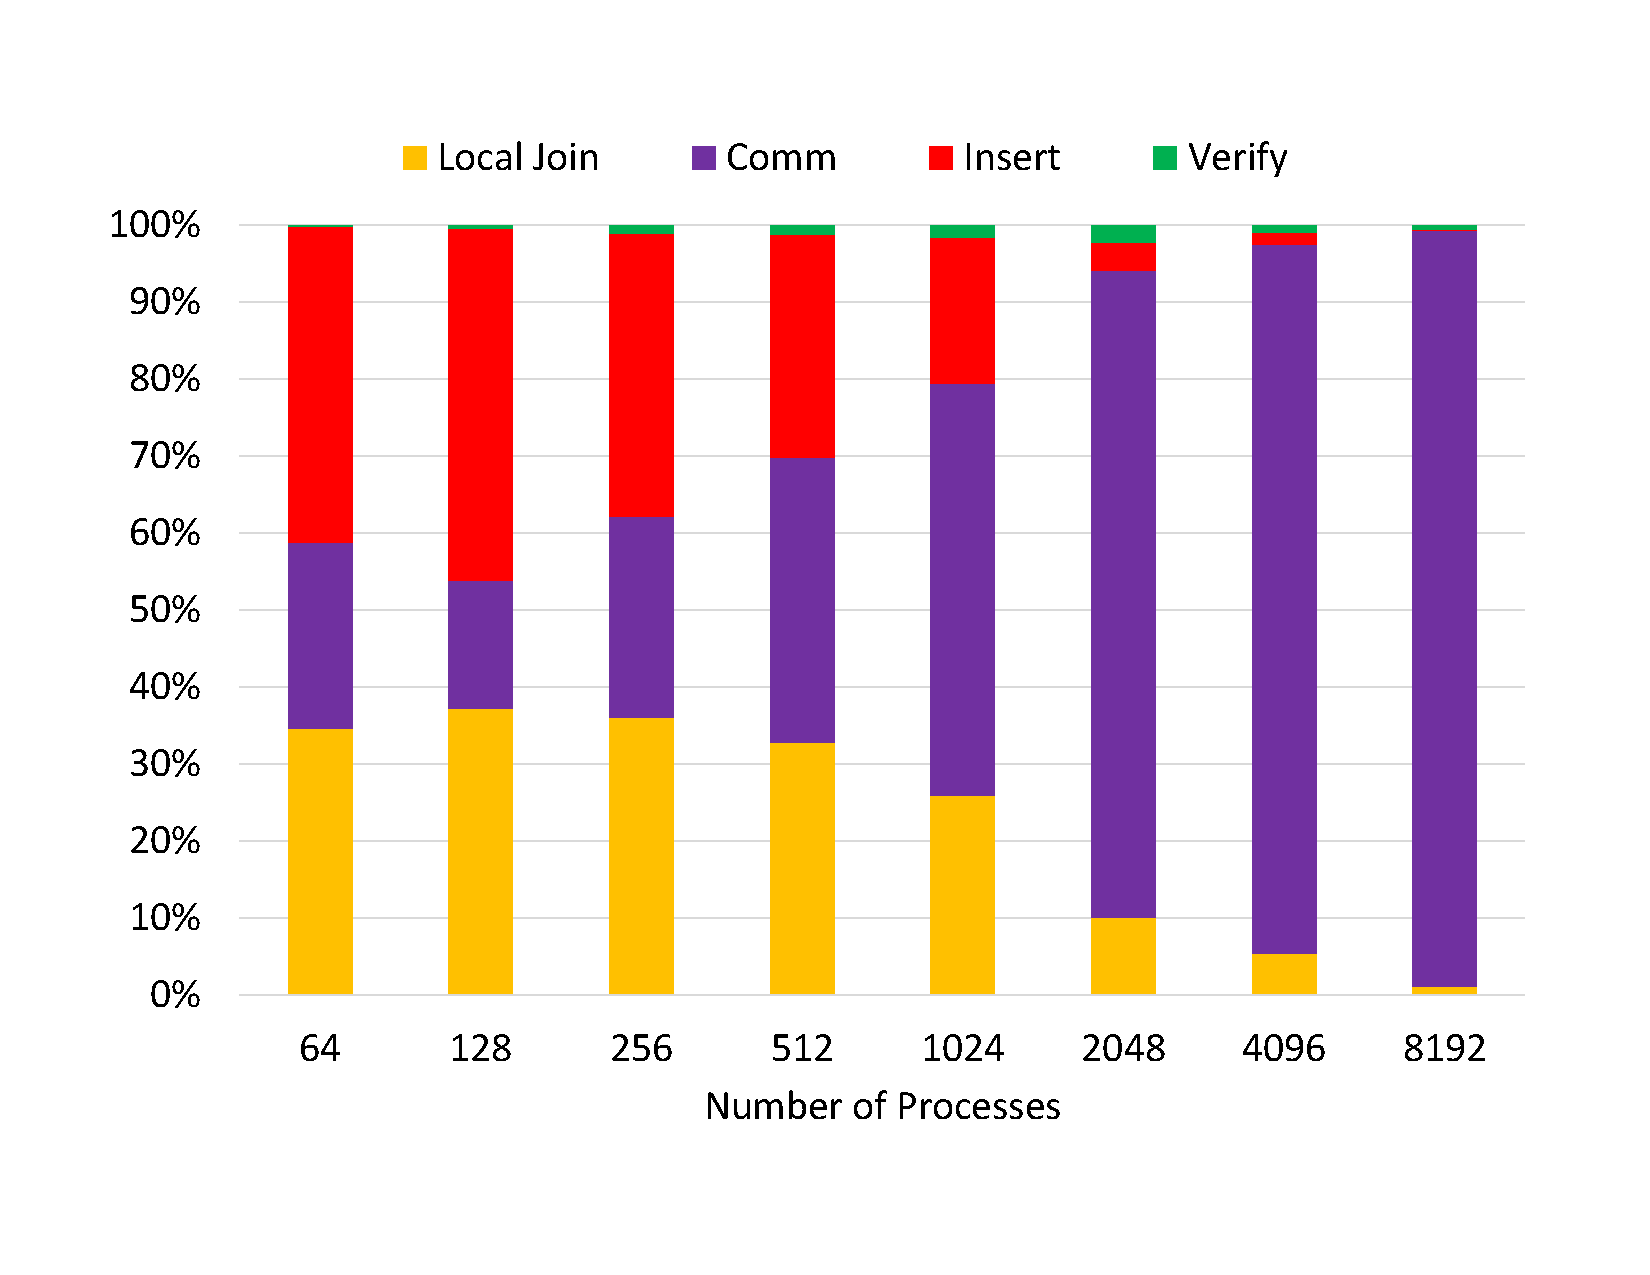
\includegraphics[width=.50\textwidth,  trim={0cm 0cm 0cm 0cm,
			clip}]{results/TC_1_break_down_final.pdf}}\hfill%
	\centering
	\caption{(Left) Strong scaling result for computing transitive closure of graph $G1$. (Right) Percentage breakdown of the four phases; communication starts to dominate after $1024$ processes. }
	\label{fig:tc_small}
\end{figure*}

\begin{figure*}[t]
	{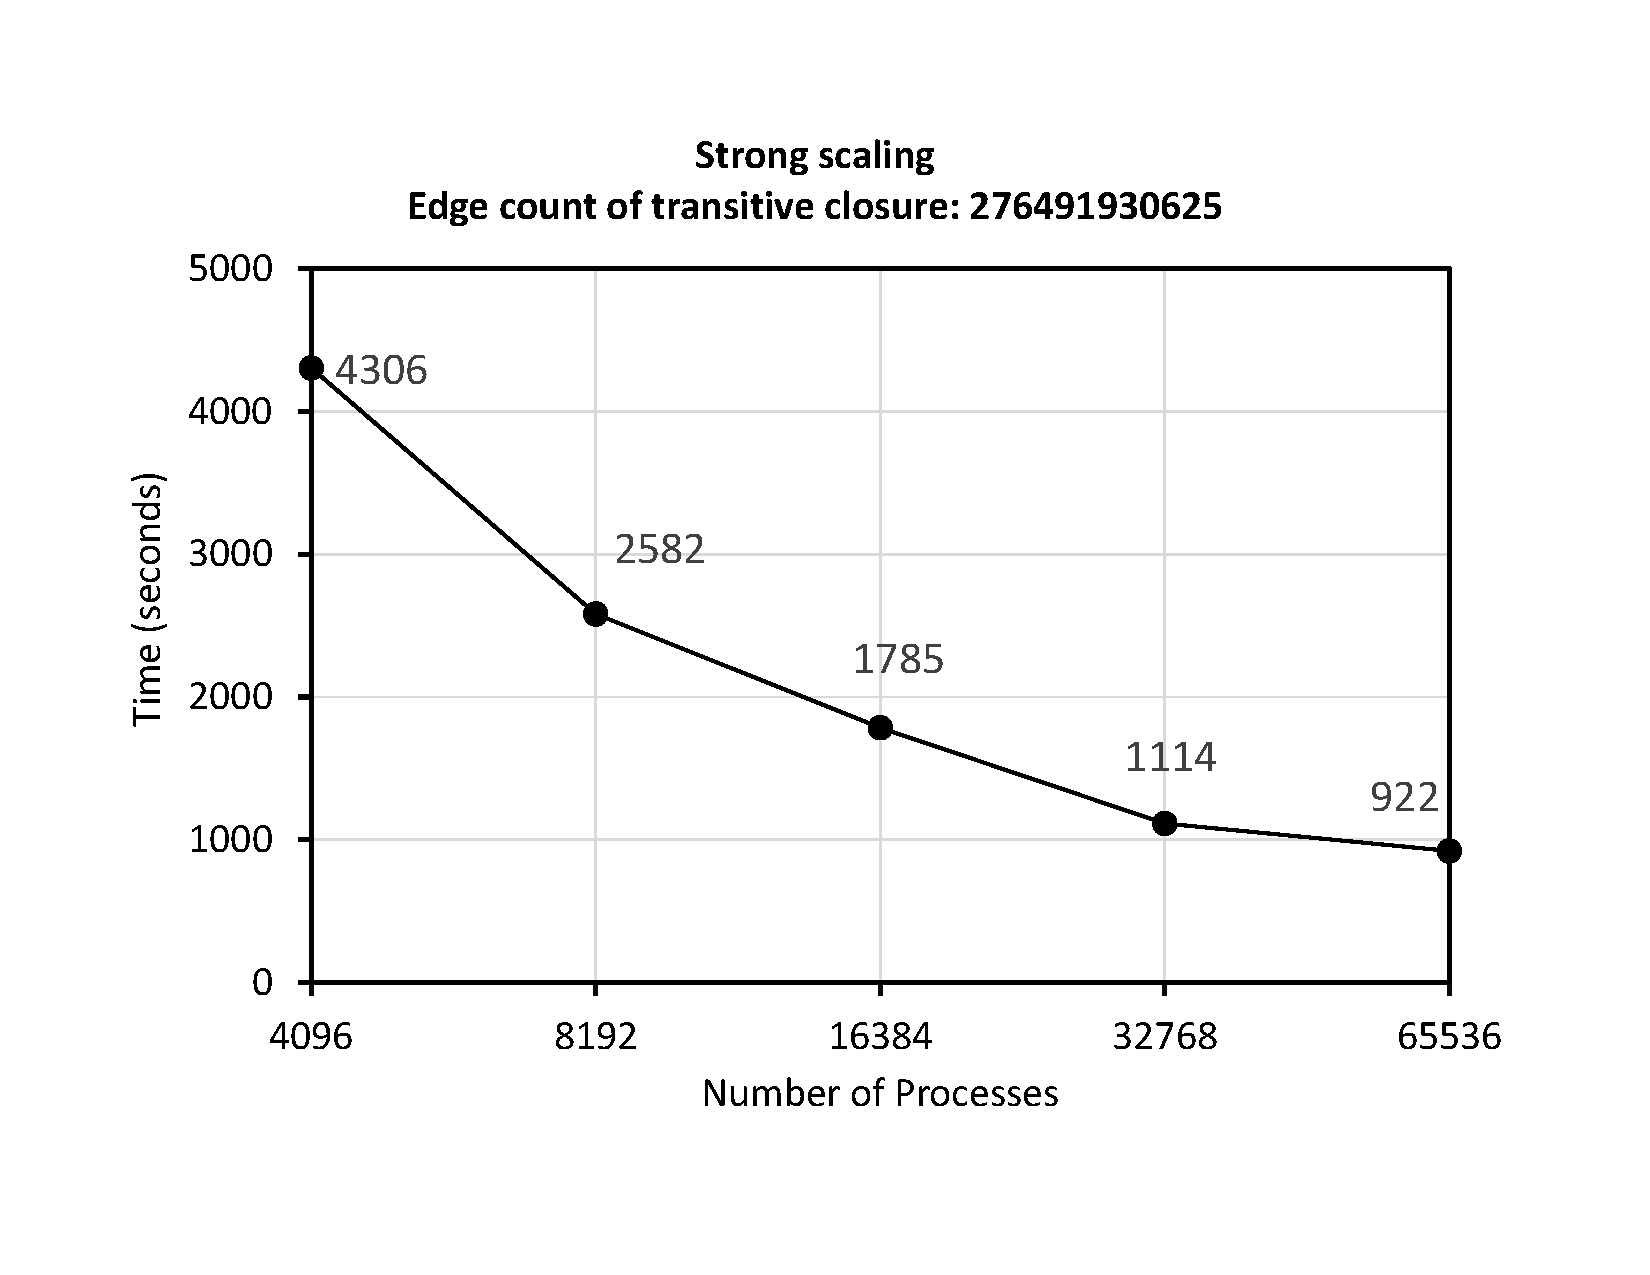
\includegraphics[width=.50\textwidth,  trim={0cm 0cm 0cm 0cm, 
			clip}]{results/TC_2_final.pdf}}\hfill%
	{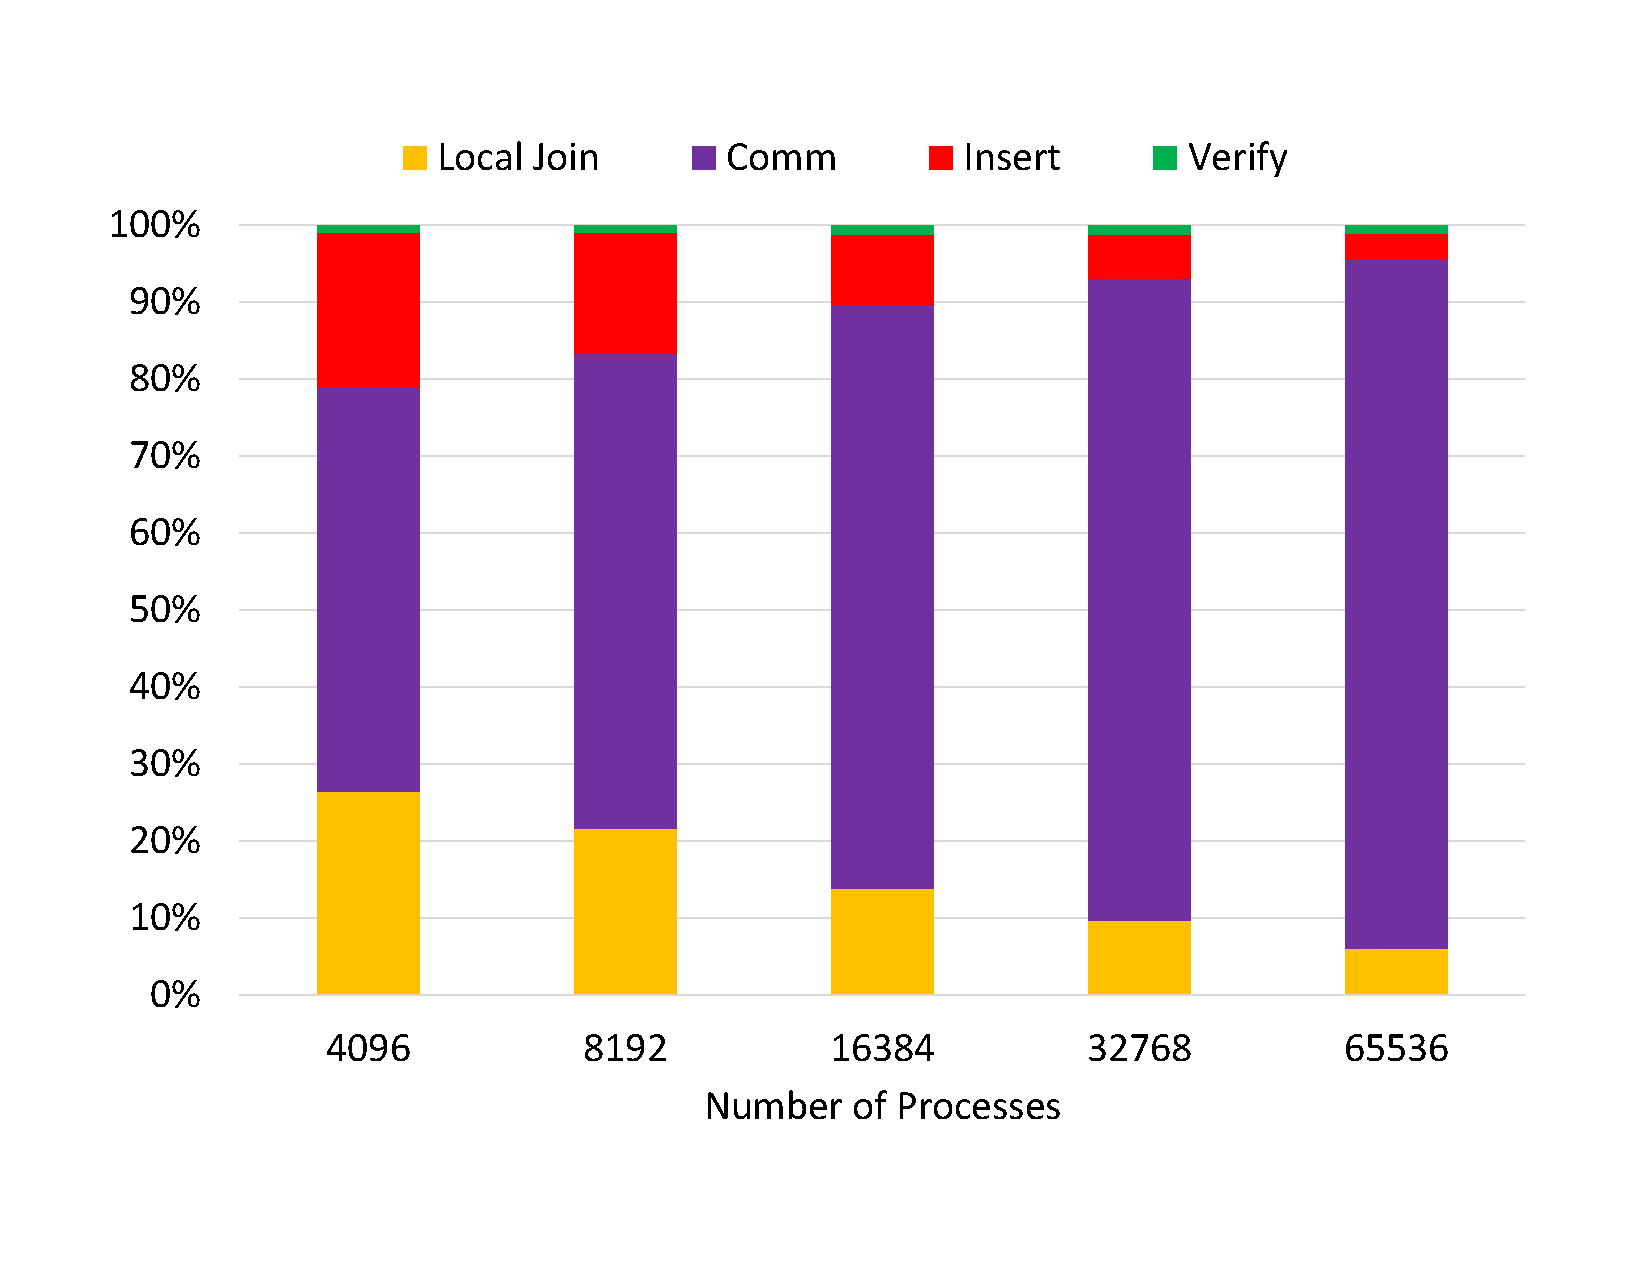
\includegraphics[width=.50\textwidth,  trim={0cm 0cm 0cm 0cm,
			clip}]{results/TC_2_break_down_final.pdf}}\hfill%
	\centering
	\caption{(Left) Strong scaling result for computing transitive closure of graph $G2$. (Right) Percentage breakdown of the four phases; communication starts to dominate after $16,384$ processes.}
	\label{fig:tc_big}
\end{figure*}


%\begin{figure*}[t]
%	{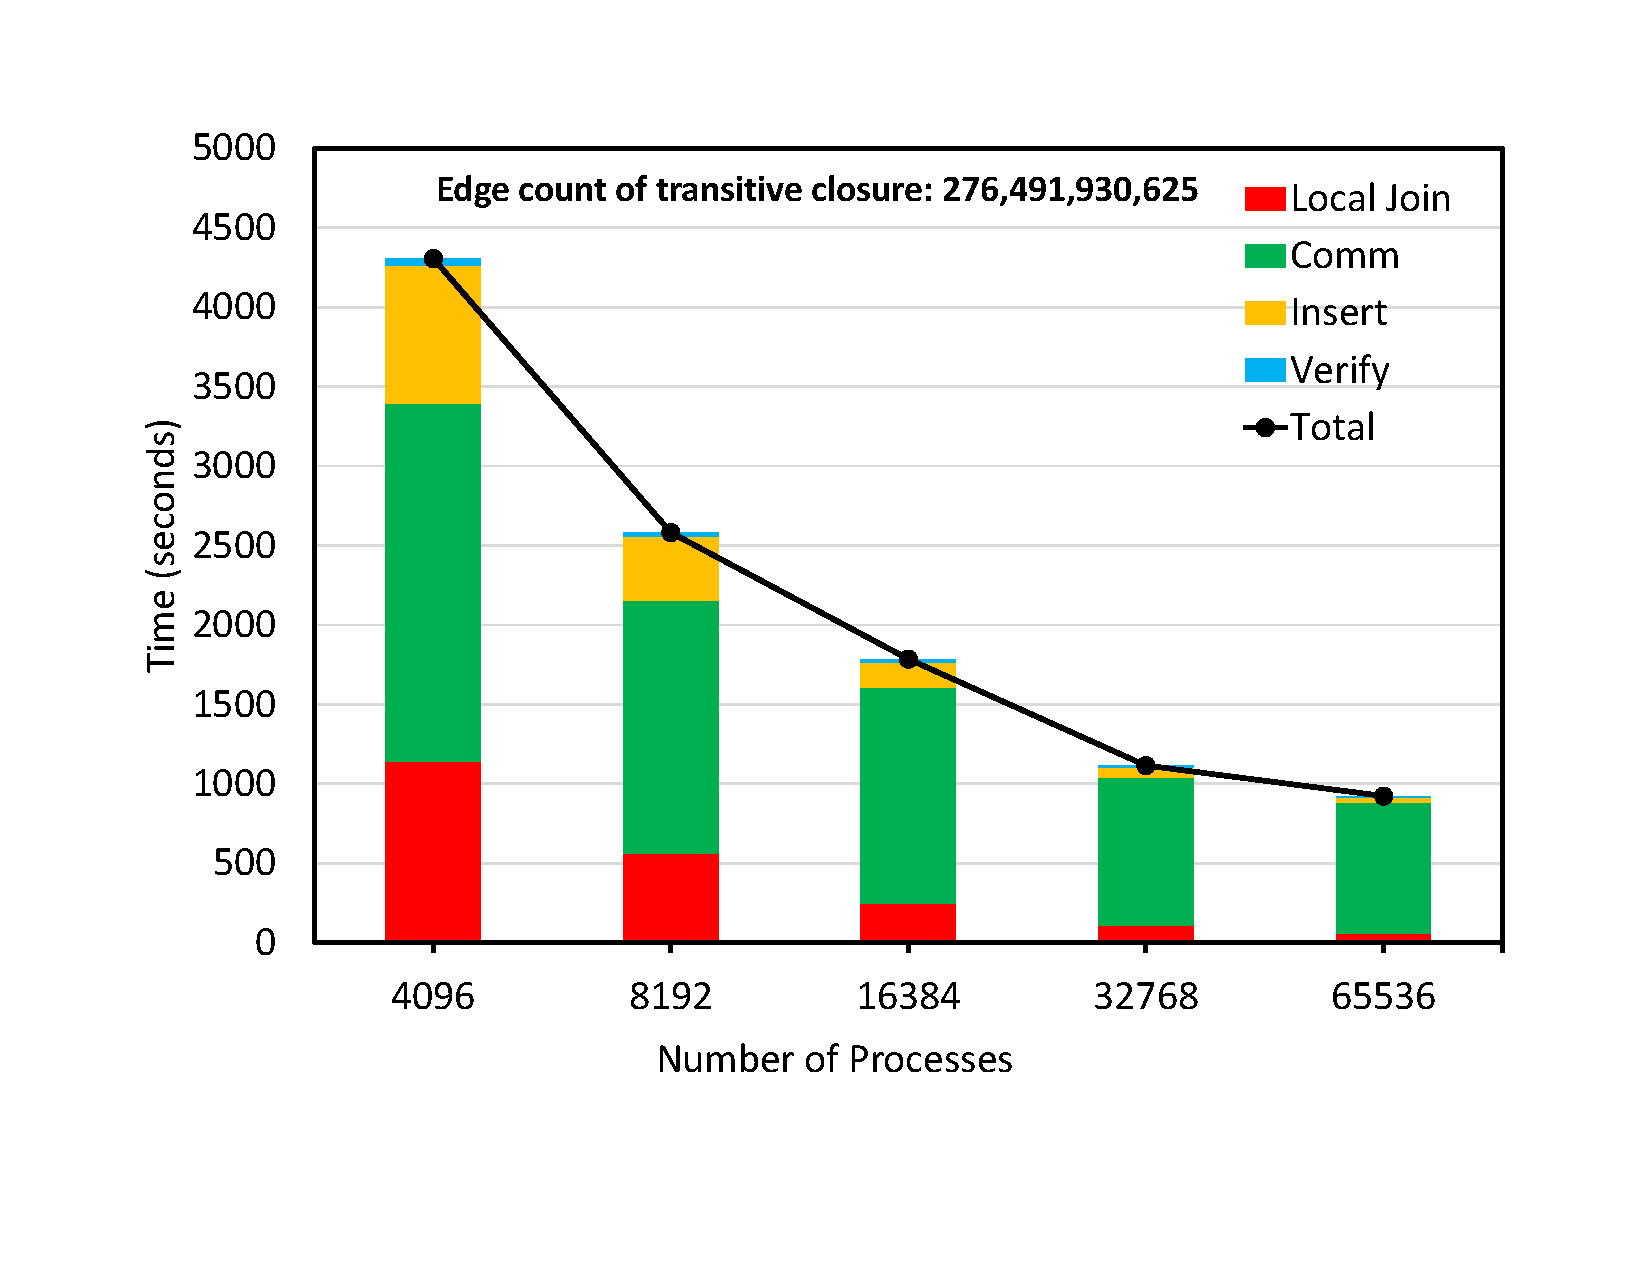
\includegraphics[width=.50\textwidth,  trim={0cm 0cm 0cm 0cm, 
%			clip}]{results/TC_260Billion_Final.pdf}}\hfill%
%	{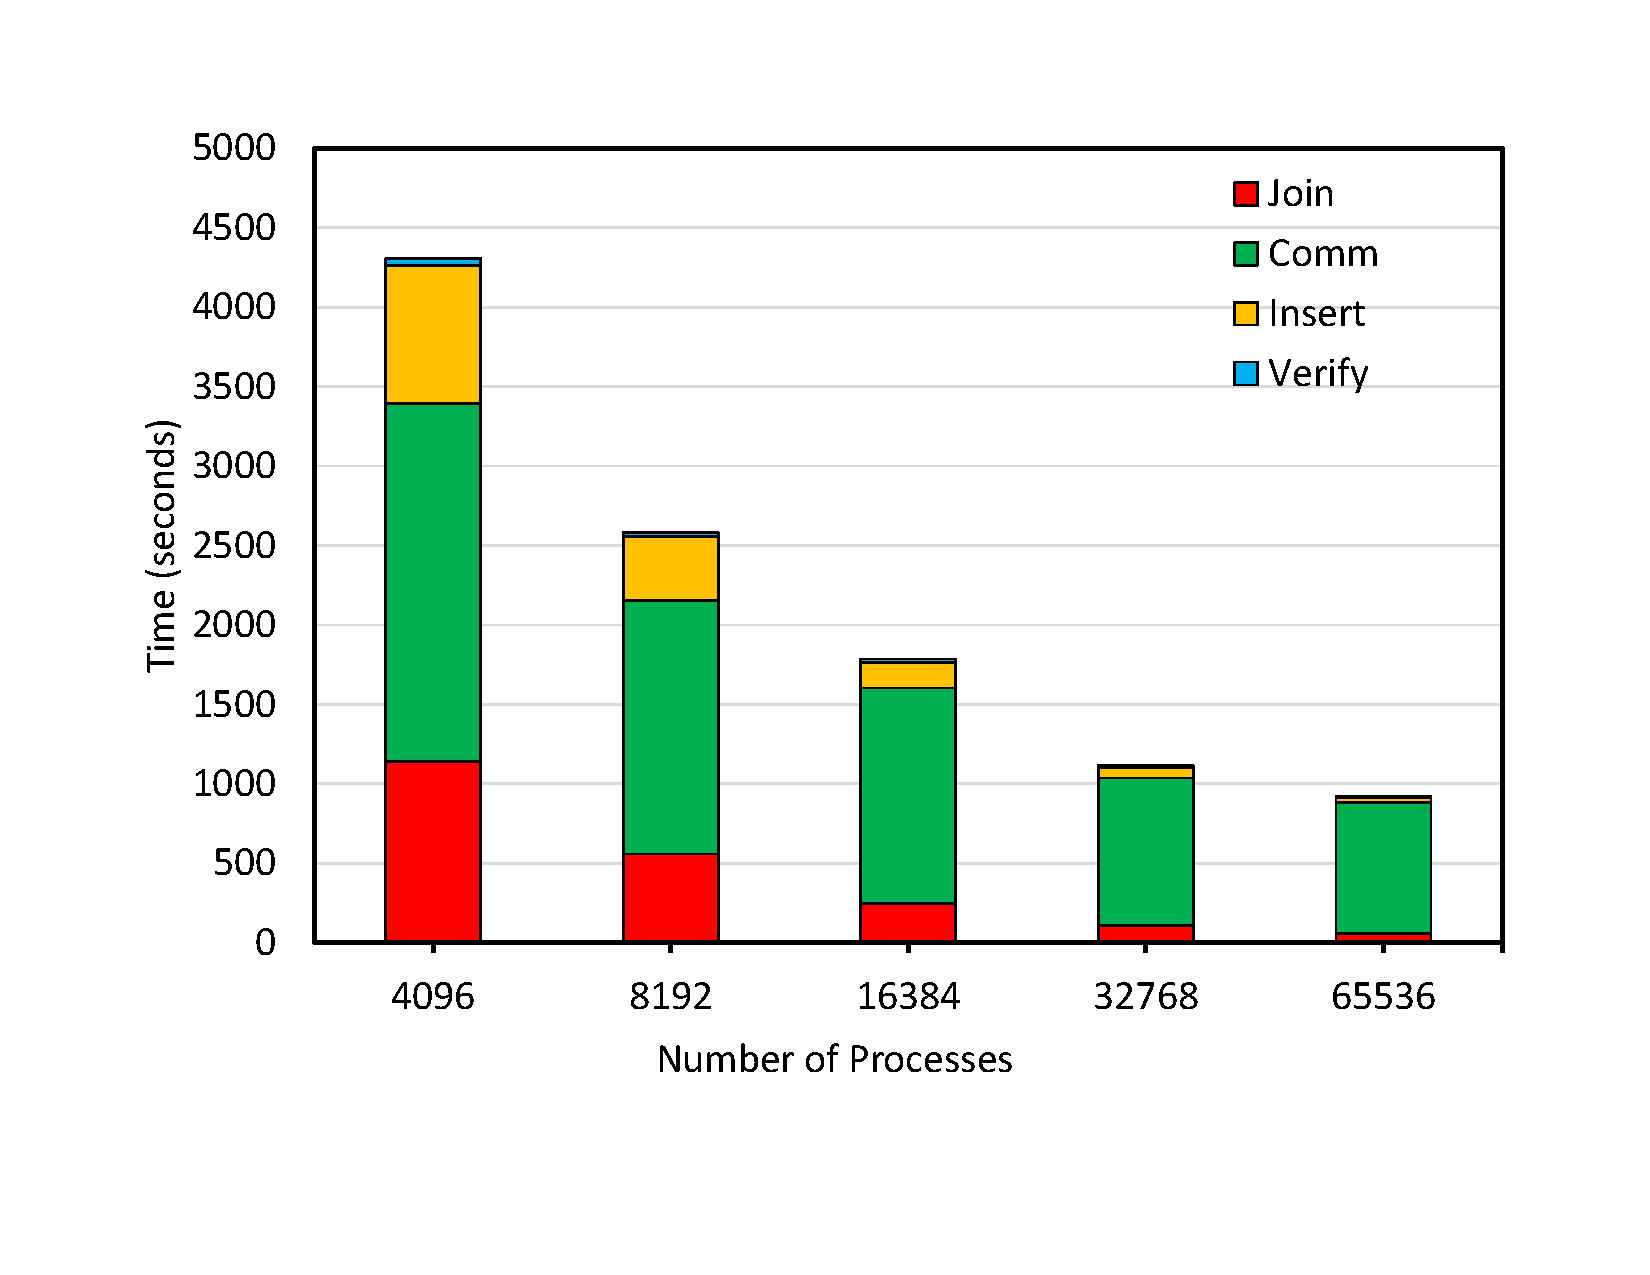
\includegraphics[width=.50\textwidth,  trim={0cm 0cm 0cm 0cm,
%			clip}]{results/TC_260Billion_breakdown.pdf}}\hfill%
%	\centering
%	\caption{Transitive closure of a graph with X edges.}
%	\label{fig:tc_large}
%\end{figure*}
